\documentclass[8pt,xcolor=table,aspectratio=169]{beamer}

\usepackage{hyperref}
\usepackage{graphicx}
\usepackage{caption}
\usepackage{subcaption}
\usepackage{transparent}
\usepackage{epstopdf} %converting to PDF
\usepackage{multicol} 
\usepackage{animate}[2017/05/18]

\usepackage{makecell}

% \usepackage{pdfx}
 
% \usepackage[utf8]{inputenc}
% \usepackage[T1]{fontenc}
\usepackage[table]{xcolor}    % loads also »colortbl« 
%  \usepackage{enumitem}
% \usepackage{ucltemplate}
\usepackage{color}

\usepackage{comment}

\usepackage{tabularx} % make width of table columns evenly distributed (see http://tex.stackexchange.com/questions/60601/evenly-distributing-column-widths)
% \newcolumntype{Y}{>{\centering\arraybackslash}X}

% make entire row bold or italic in table
\newcommand\setrow[1]{\gdef\rowmac{#1}#1\ignorespaces}
\newcommand\clearrow{\global\let\rowmac\relax}
\clearrow

\usepackage{amssymb}% http://ctan.org/pkg/amssymb
\usepackage{pifont}% http://ctan.org/pkg/pifont
\newcommand{\cmark}{\ding{51}}%
\newcommand{\xmark}{\ding{55}}%

%\usepackage{pgfgantt} % for grantt charts
\usepackage{rotating}
\usepackage[graphicx]{realboxes}
\usepackage[export]{adjustbox}
\usepackage{array}
\usepackage{bm}

%\usepackage{url}
%\usepackage{amssymb}
%\usepackage{amsthm}
%\usepackage[numbers]{natbib}
%\usepackage{enumitem}
%\usepackage{amsmath}  % required if you use \overset
%%\documentstyle[nips14submit_09,times,art10]{article} % For LaTeX 2.09
%\usepackage{array}


\usepackage{rotating}
% \usepackage{tabularx, booktabs} % make width of table columns evenly distributed (see http://tex.stackexchange.com/questions/60601/evenly-distributing-column-widths)
% \newcolumntype{Y}{>{\centering\arraybackslash}X}

\DeclareMathOperator*{\argmin}{arg\,min}
\DeclareMathOperator*{\argmax}{arg\,max}

\usepackage{tikz}
\usetikzlibrary{arrows,positioning, shapes.symbols,shapes.callouts,patterns,shapes,chains,calc,backgrounds,fadings}

% \definecolor{parCol}{rgb}{0.1, 0.1, 1}
% \definecolor{stCol}{rgb}{0.1, 0.6, 0.1}
% \definecolor{bothCol}{rgb}{0, 0.5, 0.5}

\definecolor{parCol}{rgb}{0, 0, 0}
\definecolor{stCol}{rgb}{0, 0, 0}
\definecolor{bothCol}{rgb}{0, 0, 0}
\definecolor{blue3}{HTML}{86B7FC} % med blue
\definecolor{blue1}{HTML}{B5F1FF} % light blue
\definecolor{blue2}{HTML}{E0F9FF} % very light blue

\newcolumntype{C}[1]{>{\centering\let\newline\\\arraybackslash\hspace{0pt}}m{#1}}

\setlength{\tabcolsep}{0.2em}

 
 %% OVERVIEW OF WORK SO FAR %%
 
%Information to be included in the title page:
\title{Tutorial on Generative Adversarial Networks  - From basics to current state-of-the-art, and towards key applications in medicine}
\author[Raz]{
R\u{a}zvan V. Marinescu\vspace{1em}}

\institute{\small{Medical Vision Group, Massachusetts Institute of Technology}

%\vspace{0em}
%\small{Centre for Medical Image Computing, University College London, UK}
}

\date{}

% logo of my university
\titlegraphic{
   \begin{figure}
%   \begin{subfigure}{0.32\textwidth}
%   \hspace{2em}
%   
\includegraphics[height=1.0cm]{ucl_logo}
%   \end{subfigure}
   \begin{subfigure}{0.32\textwidth}
   \centering
   
\includegraphics[height=1.0cm]{MIT_logo.png} 
   \end{subfigure}

   \end{figure}
   
   \tiny{Slides available online: https://people.csail.mit.edu/razvan}
}

\setbeamercolor{frametitle}{fg=black}
\setbeamercolor{author in head/foot}{fg=black, bg=white} 
\setbeamercolor{institute in head/foot}{fg=black, bg=white} 
\setbeamercolor{title in head/foot}{fg=black, bg=white}
\setbeamercolor{date in head/foot}{fg=black, bg=white}

\setbeamersize{text margin left=10pt,text margin right=10pt}
% \setbeamertemplate{frametitle}{
%     \vspace{0.9em}
%     \insertframetitle
% %     \vspace{-3em}
% }
\setbeamertemplate{frametitle}{%
    \vspace{0.5em}
    \usebeamerfont{frametitle}\insertframetitle%
    \vphantom{g}% To avoid fluctuations per frame
    %\hrule% Uncomment to see desired effect, without a full-width hrule
    \par% <-- added
    \hspace*{-\dimexpr0.5\paperwidth-0.5\textwidth}% <-- calculation of left margin width
    \rule[0.5\baselineskip]{\paperwidth}{0.4pt}%
}

\setbeamertemplate{footline}
{
  \vspace{-3em}
  \leavevmode%
   \rule{\paperwidth}{0.3pt}
  \hbox{%
  \begin{beamercolorbox}[wd=.3\paperwidth,ht=2.25ex,dp=1ex,center]{author in head/foot}%
    \usebeamerfont{author in head/foot}Razvan V. Marinescu
  \end{beamercolorbox}%
  \begin{beamercolorbox}[wd=.3\paperwidth,ht=2.25ex,dp=1ex,center]{institute in head/foot}%
    \usebeamerfont{institute in head/foot}razvan@csail.mit.edu
  \end{beamercolorbox}%
  \begin{beamercolorbox}[wd=.3\paperwidth,ht=2.25ex,dp=1ex,center]{institute in head/foot}%
    \usebeamerfont{institute in head/foot}https://people.csail.mit.edu/razvan/
  \end{beamercolorbox}%
%   \begin{beamercolorbox}[wd=.2\paperwidth,ht=2.25ex,dp=1ex,center]{title in head/foot}%
%     \usebeamerfont{title in head/foot}\insertsection
%   \end{beamercolorbox}%
  \begin{beamercolorbox}[wd=.10\paperwidth,ht=2.25ex,dp=1ex,right]{date in head/foot}%
    \usebeamerfont{date in head/foot}\insertshortdate{}\hspace*{2em}
    \insertframenumber{} / \inserttotalframenumber\hspace*{2ex}
  \end{beamercolorbox}}%
  \vskip0pt%
}

% \usepackage{beamerthemesplit}

\newcommand{\backupbegin}{
   \newcounter{finalframe}
   \setcounter{finalframe}{\value{framenumber}}
}
\newcommand{\backupend}{
   \setcounter{framenumber}{\value{finalframe}}
}


\makeatletter
\long\def\beamer@author[#1]#2{%
  \def\and{\tabularnewline}
  \def\insertauthor{\def\inst{\beamer@insttitle}\def\and{\tabularnewline}%
  \begin{tabular}{rl}#2\end{tabular}}%
  \def\beamer@shortauthor{#1}%
  \ifbeamer@autopdfinfo%
    \def\beamer@andstripped{}%
    \beamer@stripands#1 \and\relax
    {\let\inst=\@gobble\let\thanks=\@gobble\def\and{, }\hypersetup{pdfauthor={\beamer@andstripped}}}
  \fi%
}
\makeatother
\beamertemplatenavigationsymbolsempty
\setbeamertemplate{caption}[numbered]
\setbeamercolor{caption name}{fg=black}
\setbeamercolor{itemize item}{fg=black}
\setbeamercolor{itemize subitem}{fg=black}
\setbeamercolor{enumerate item}{fg=black}
\setbeamercolor{enumerate subitem}{fg=black}
\setbeamertemplate{enumerate item}[default]
\setbeamertemplate{enumerate subitem}[default]

\makeatletter
\let\@@magyar@captionfix\relax
\makeatother
\begin{document}
 
\section{Introduction}

\frame{\titlepage}
 
\setbeamerfont{frametitle}{size=\large}

%\newcommand{\upgradeReportLoc}{../../upgrade_report}
%\newcommand{\epsrcPresLoc}{\upgradeReportLoc/epsrcPres}
%\newcommand{\jointModellingDiseaseLoc}{../../jointModellingDisease}
%\newcommand{\pcaLongPaperLoc}{../../PCA_long_paper}
%\newcommand{\voxFld}{../../voxelwiseDPM}
%\newcommand{\tadpoleFld}{../../tadpole}
%\newcommand{\diffEqModelFld}{../../diffEqModel}



%\newcommand*{\pcaLongFigs}{\pcaLongPaperLoc/figures}


% \includeonlyframes{1-20}
%\includeonlyframes{current}


\definecolor{light-gray}{gray}{0.6}



\begin{frame}{Generative adversarial networks}
 
 \begin{itemize}
 
\item GAN basics
  
  \vspace{2em}
  
\item State-of-the-art
  
  \vspace{2em}
    
\item Key applications in computer vision and medicine
  
  \vspace{2em}

\item Preliminary results on three different medical datasets
  
 \end{itemize}

\end{frame}

\begin{frame}{Introduction to Generative Models}

\begin{columns}
\begin{column}{0.5\textwidth}

\begin{itemize}
 \item Generative: can generate new data instances
 
 $$ p(X,Y) $$
 
 \item Discriminative: discriminates between different kinds of data instances
 
 $$ p(Y|X) $$
 

 $X$ = image\\
 $Y$ = label/score
 

\end{itemize}

\end{column}
\begin{column}{0.5\textwidth}
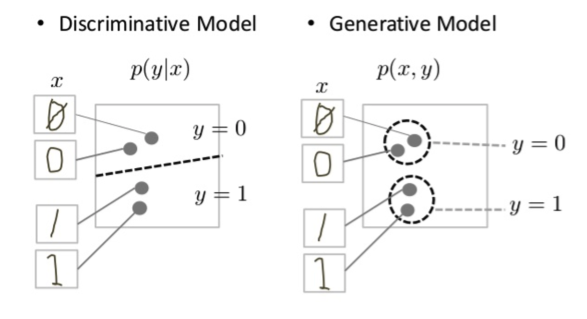
\includegraphics[width=\textwidth]{YM8rTF1.png} 

\end{column}
\end{columns}

\end{frame}

\begin{frame}{Introduction to Generative Adversarial Networks}



\begin{columns}
\begin{column}{0.5\textwidth}

\begin{itemize}
 \item Introduced by Goodfellow et al, 2014

 \vspace{2em}

 \item Two adversaries (generator + discriminator) compete with each other

 \vspace{2em}

 \item Over time, the generator gets better at generating images
 
\end{itemize}

\end{column}
\begin{column}{0.5\textwidth}
\vspace{-3em}
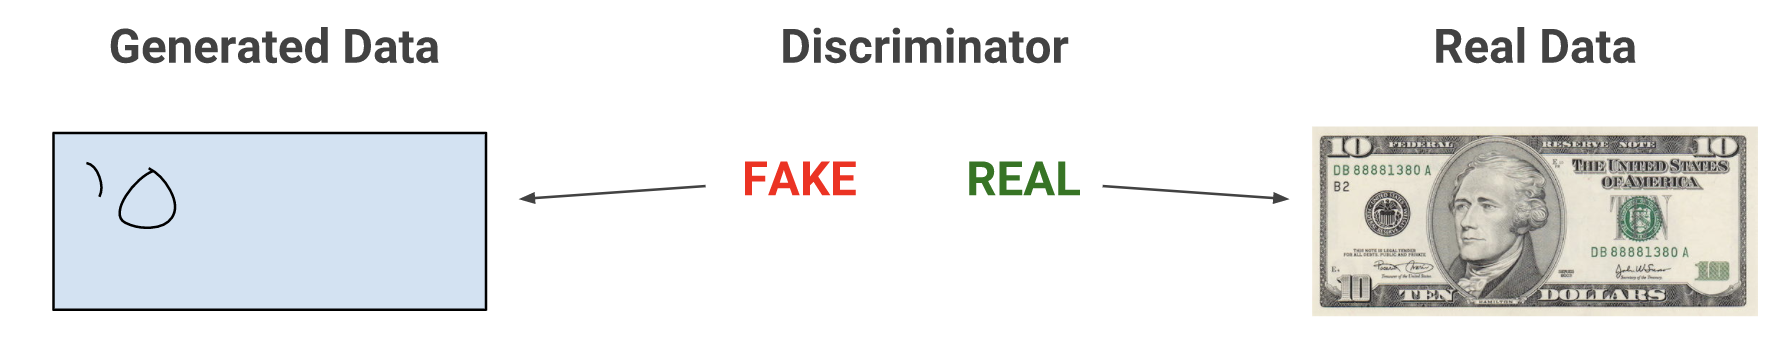
\includegraphics[width=\textwidth]{8EREjP8.png} 

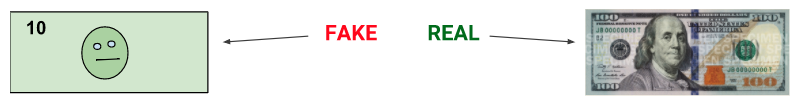
\includegraphics[width=\textwidth]{qocPf9V.png}\\ 

\begin{center}
...\\
\end{center}

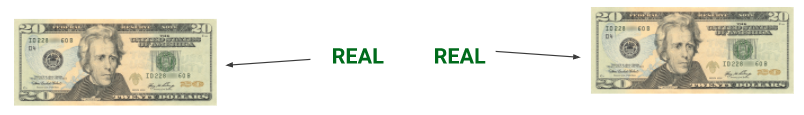
\includegraphics[width=\textwidth]{p3KwCvb.png} 


\end{column}
\end{columns}
  
 
 \end{frame}
 
\begin{frame}{GAN architecture}

\begin{itemize}
  \item Generator attempts to generate good images to fool the discriminator
  \item Discriminator attempts to tell apart the fake images from the real ones
  \item Loss function:
$$\min_G \max_D V(D, G) = \mathbb{E}_{\bm{x} \sim p_{\text{data}}(\bm{x})}[\log D(\bm{x})] + \mathbb{E}_{\bm{z} \sim p_{\bm{z}}(\bm{z})}[\log (1 - D(G(\bm{z})))].
$$
\end{itemize}

\begin{figure}
\centering
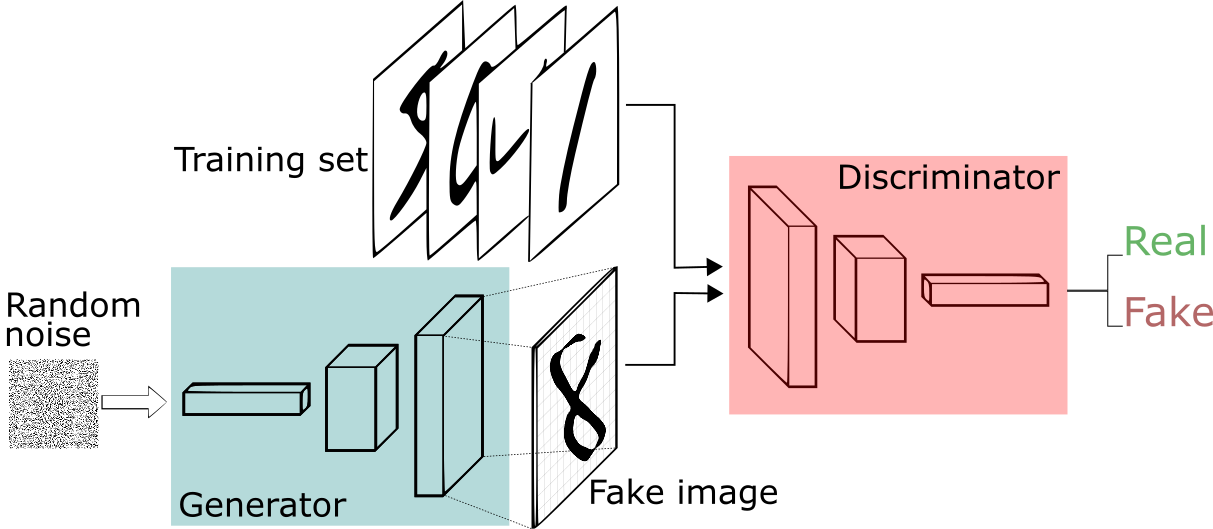
\includegraphics[width=0.7\textwidth]{gan}\\
\vspace{2em}


\end{figure}
\end{frame}

\begin{frame}[plain, c]

\begin{center}
\Huge Towards the state-of-the-art in Generative Adversarial Networks
\end{center}

\end{frame}

\begin{frame}{Initial GAN results (DCGAN, Radford et al, 2015)}

\begin{columns}
\begin{column}{0.5\textwidth}

\begin{itemize}
\item Initial results looked promising, but still a long way from photorealism

\vspace{2em}

\item Other problems persisted:
\begin{itemize}
\item Training collapse
\item Mode collapse
\item Low coverage

\end{itemize}

\vspace{2em}

\item Dynamics between G \& D not well understood

\end{itemize}

\end{column}
\begin{column}{0.5\textwidth}
\centering
%\vspace{-0.5em}
Standard samples\\
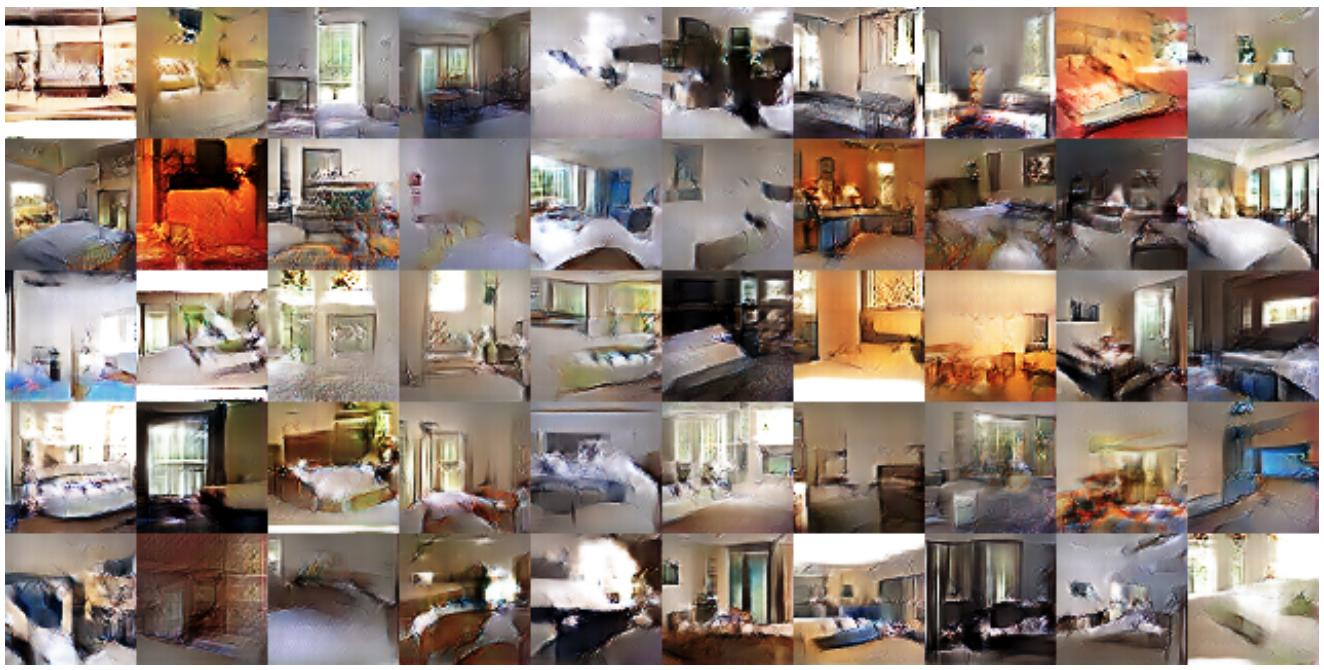
\includegraphics[width=0.75\textwidth]{ayYEUKy.jpg}
\vspace{0.5em}

Training collapse\\
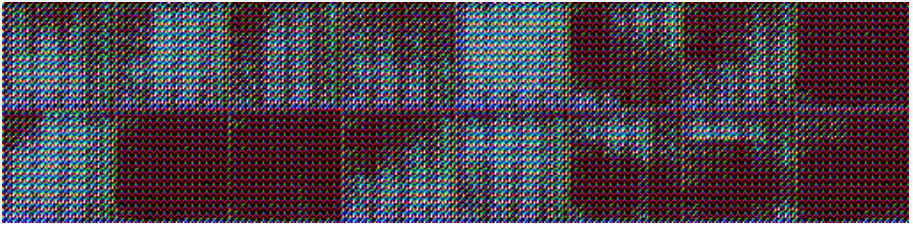
\includegraphics[width=0.75\textwidth]{fw7jvWk.png}
\vspace{0.5em}

Mode collapse\\
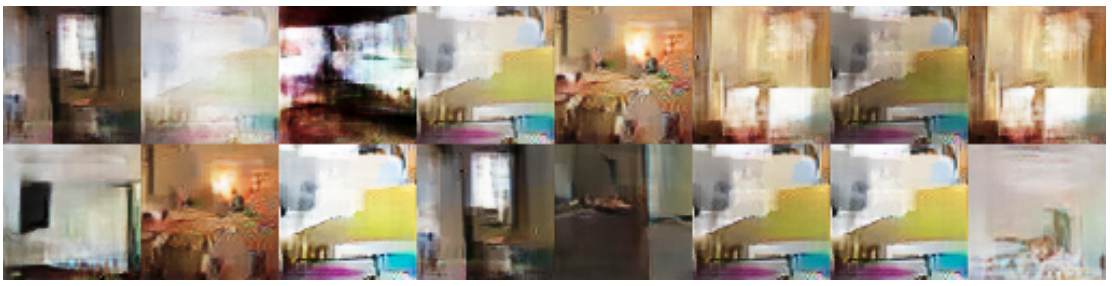
\includegraphics[width=0.75\textwidth]{QSBCbu0.png}

\end{column}
\end{columns}

\end{frame}

\begin{frame}{Wasserstein GANs (Arjovski et al, 2017)}


\begin{columns}
\begin{column}{0.5\textwidth}

\begin{itemize}
\item Original GANs were very hard to train

\vspace{2em} 

\item Problem: They optimise the Jensen-Shannon divergence, a ``vertical`` distance $\to$ no good gradients when distributions far away
 
\vspace{2em} 
 
\item A``horizontal`` distance (e.g. Wasserstein) ensures gradients are non-zero when distributions don't have support (i.e. far away)
 
 \vspace{2em} 
 
 \item GAN trained with the new Wasserstein metric collapses less often, and generates better images
 
% \item Fixed mode collapse through minibatch std

\end{itemize}

\end{column}
\begin{column}{0.5\textwidth}
\centering
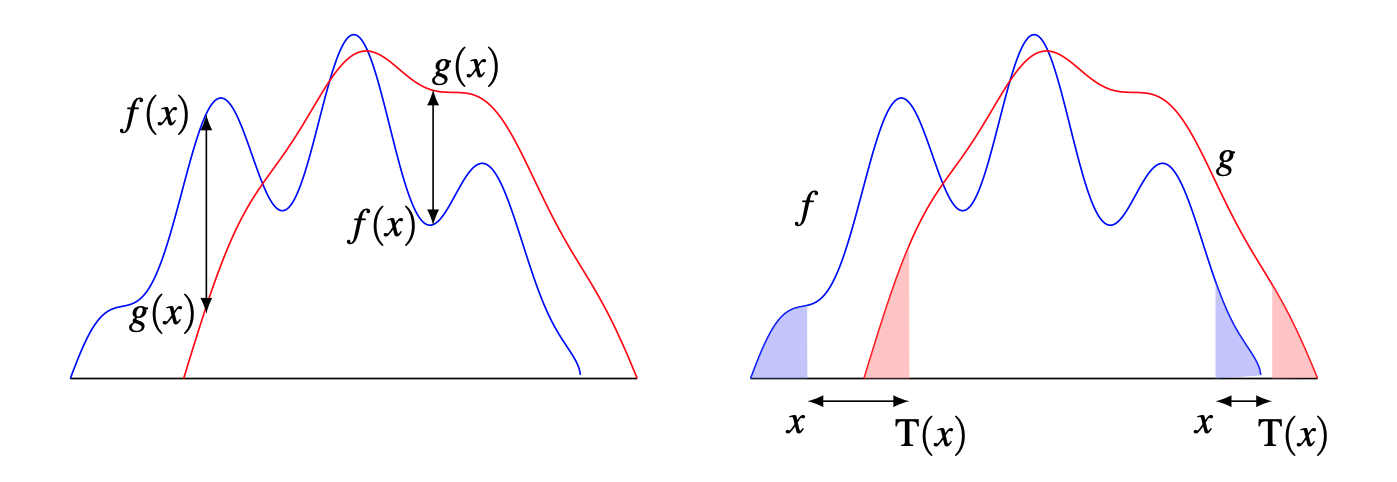
\includegraphics[width=\textwidth]{wasserstein}

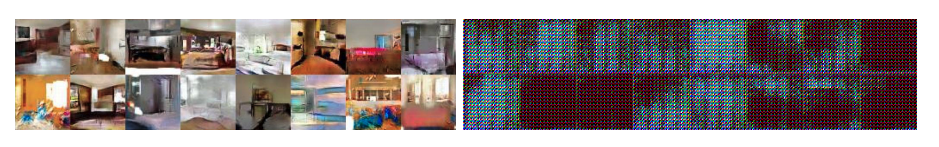
\includegraphics[width=\textwidth]{nMnEATk.png}


\end{column}
\end{columns}
  

\end{frame}

\begin{frame}{Progressive Growing of GANs (Karras et al, 2018)}
\begin{columns}
\begin{column}{0.5\textwidth}
\begin{itemize}
 \item GAN training unstable if one starts directly in high-resolution
 
 \vspace{2em} 
 
 \item Key idea: start from low-resolution (4x4) and build up to highest-resolution (1024x1024)
 
 \vspace{2em} 
 
 \item Each new layer is faded-in slowly
\end{itemize}
\end{column}
\begin{column}{0.5\textwidth}
\centering
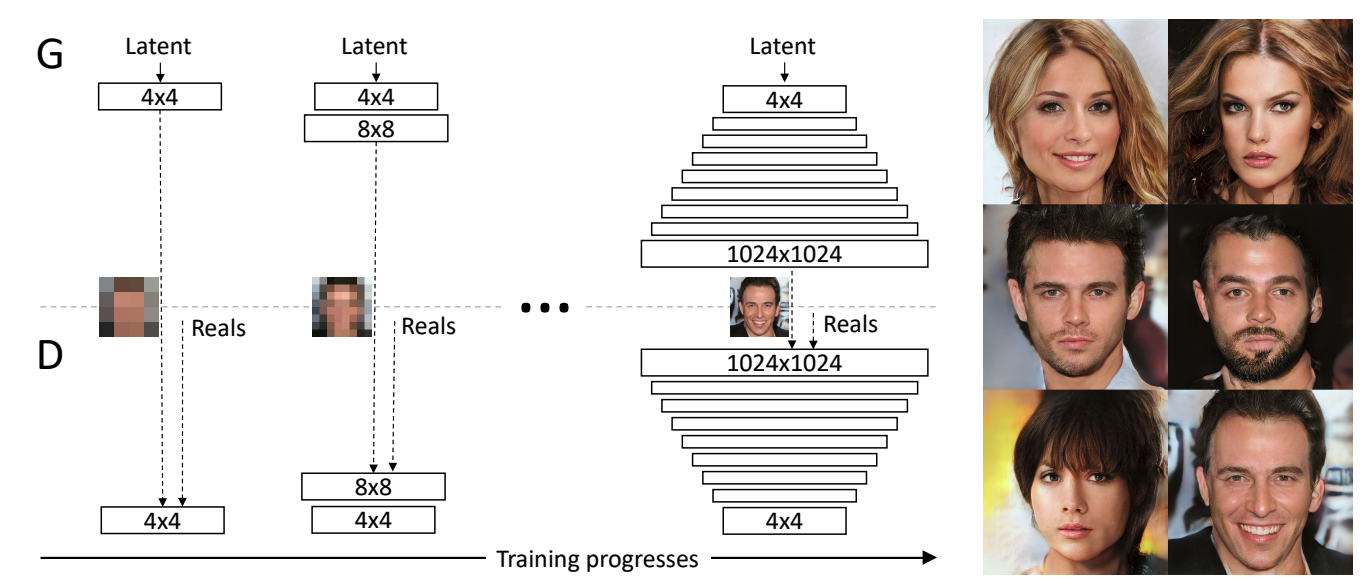
\includegraphics[width=\textwidth]{ZzLPY30.png}

\vspace{2em}

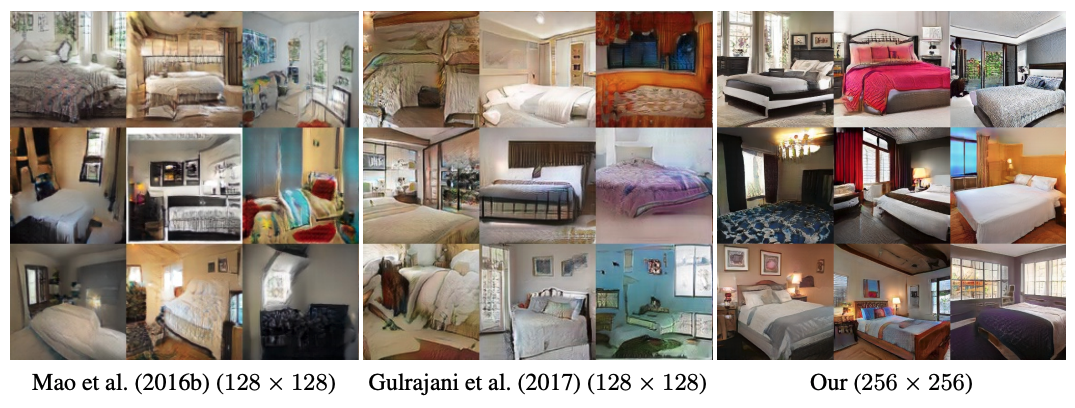
\includegraphics[width=\textwidth]{CP4yMsg.png}
%(Karras et al, 2018)
\end{column}
\end{columns}

\end{frame}

\begin{frame}{StyleGAN1 (Karras et al, 2019)}

\begin{columns}
\begin{column}{0.5\textwidth}

\begin{itemize}
 \item Borrows ideas from style-transfer literature 
 
 \vspace{0.5em} 
 
 \item Uses a mapping network to generate ``style vectors`` at every level in the generator

 \vspace{0.5em} 
 
 \item Each style vector is intensity-normalized (AdaIN operation)
 
 \vspace{0.5em}
 
 \item Generated images have unprecedented realism and diversity

\end{itemize}

\begin{center}
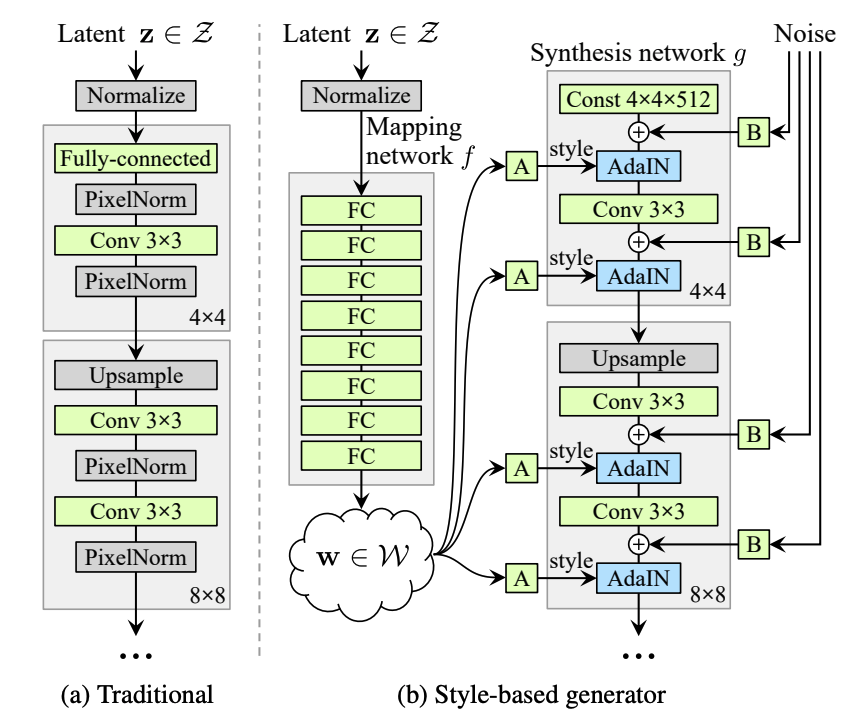
\includegraphics[width=0.6\textwidth]{qvLyFbU.png}
\end{center}

\end{column}
\begin{column}{0.5\textwidth}
\centering
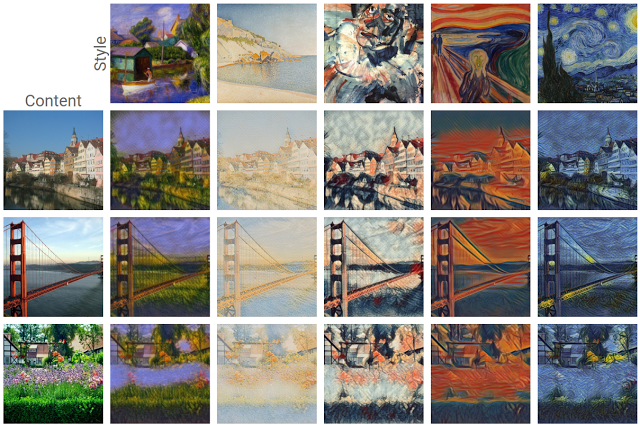
\includegraphics[width=0.7\textwidth]{style}

\vspace{2em}

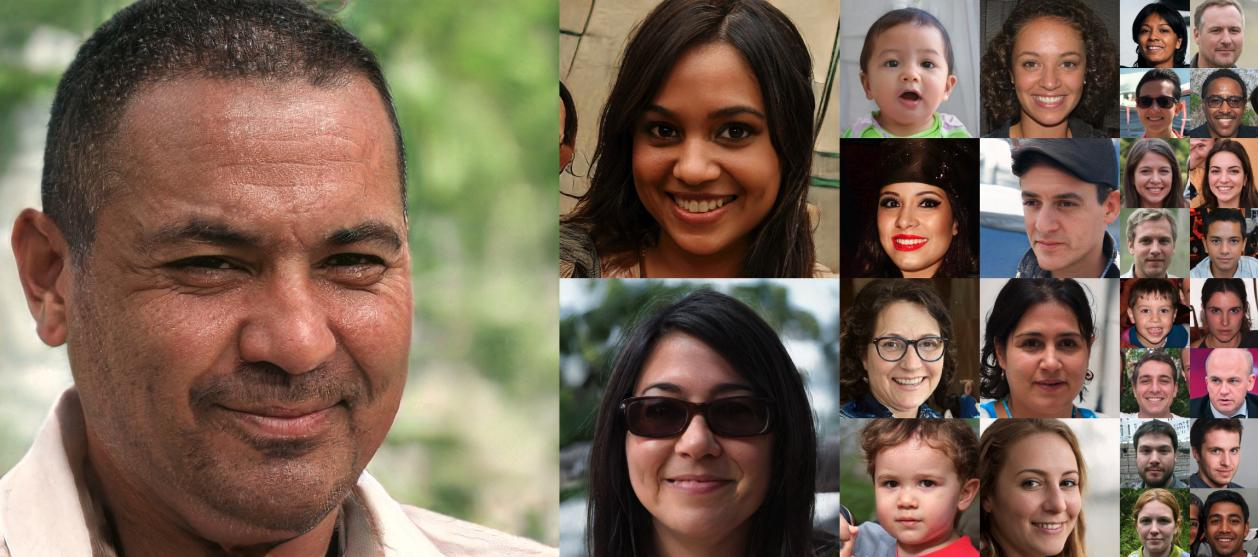
\includegraphics[width=\textwidth]{y5fwzHL.jpg}
%(Karras et al, 2019)

\end{column}
\end{columns}

\end{frame}

\begin{frame}{The style-based architecture allows both style-transfer and fine-level stochastic variation}

\begin{columns}
\begin{column}{0.6\textwidth}
\centering
Style-transfer
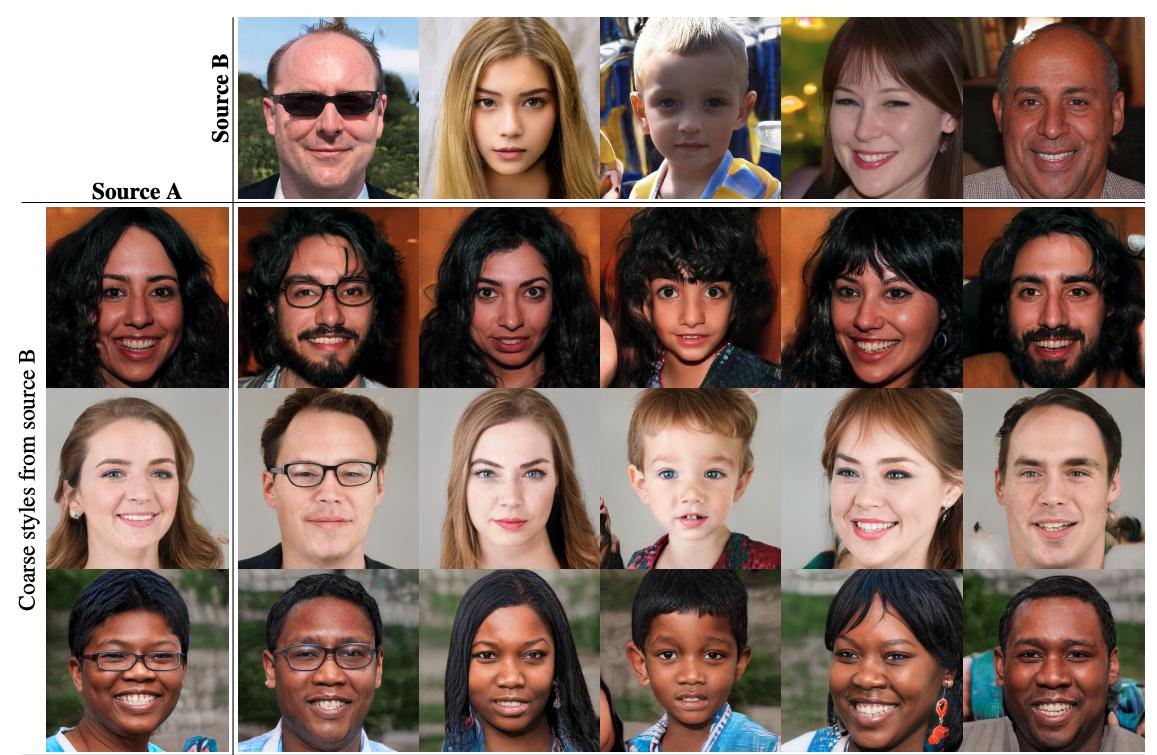
\includegraphics[width=\columnwidth]{Afh1Rkf.jpg}

\end{column}
\begin{column}{0.4\textwidth}
\centering
Fine-level stochastic variation
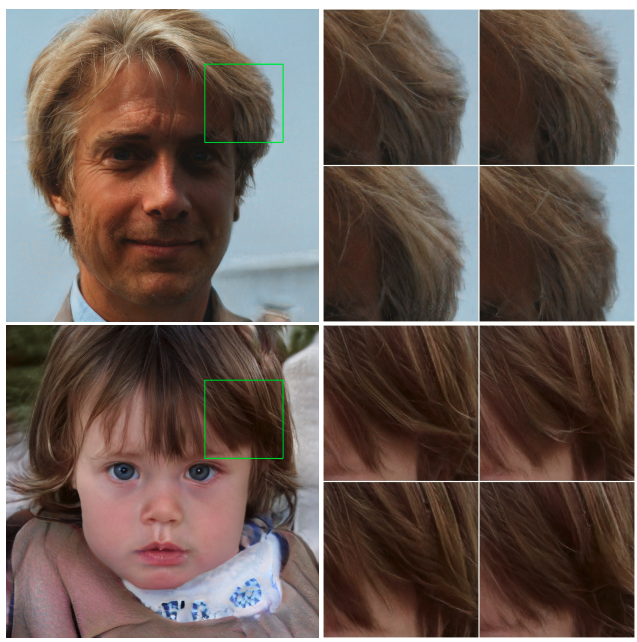
\includegraphics[width=\columnwidth]{VGY5xB7.png}

\end{column}
\end{columns}
\end{frame}

\begin{frame}{StyleGAN2 improvements (Karras et al, 2019b)}


\begin{columns}[t]
\begin{column}{0.6\textwidth}
\centering
Blob-artefacts caused by AdaIN normalisation
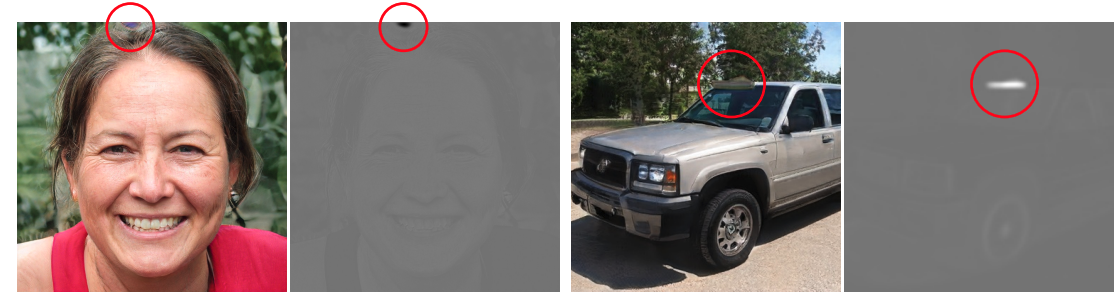
\includegraphics[width=\columnwidth]{LM3Ox5i.png}

\vspace{2em}

Solution: bake normalisation straight into convolution weights:

$$w''_{ijk} = w'_{ijk} \bigg/ \sqrt{\raisebox{0mm}[4.0mm][2.5mm]{$\underset{i,k}{{}\displaystyle\sum{}}$} {w'_{ijk}}^2 + \epsilon} $$
\end{column}
\begin{column}{0.4\textwidth}
\centering
``phase`` artefacts due to progressive growing
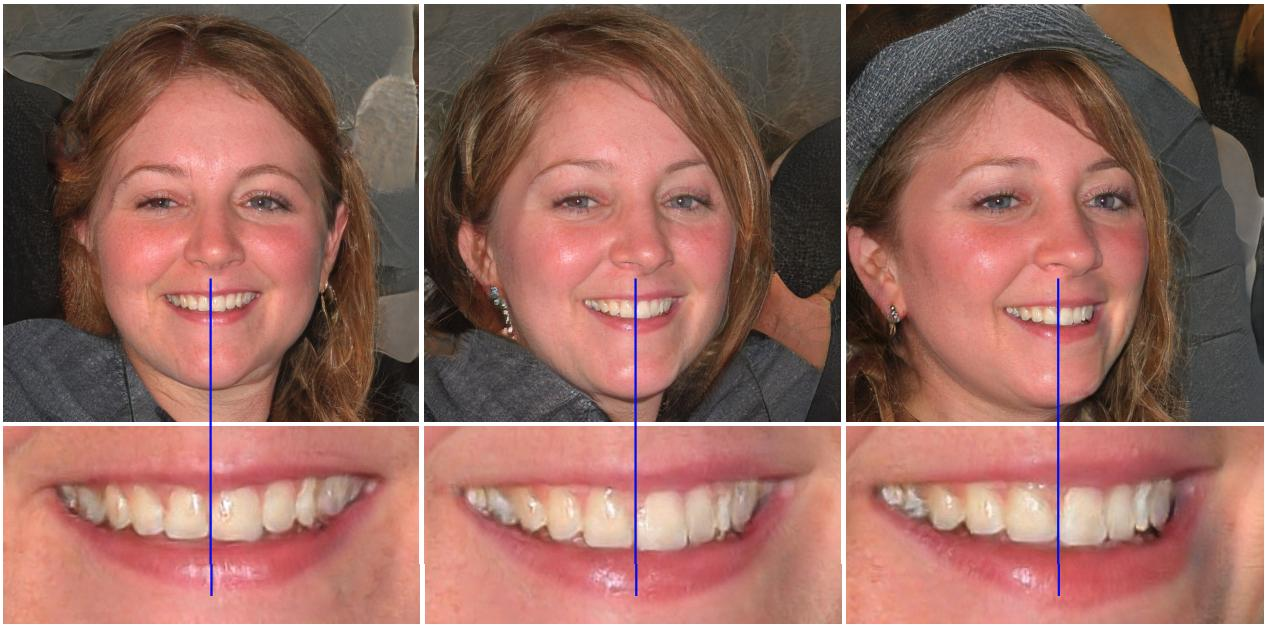
\includegraphics[width=\columnwidth]{mTWHXPW.jpg}

\vspace{2em}
Solution: communicate across resolution levels through skip connections
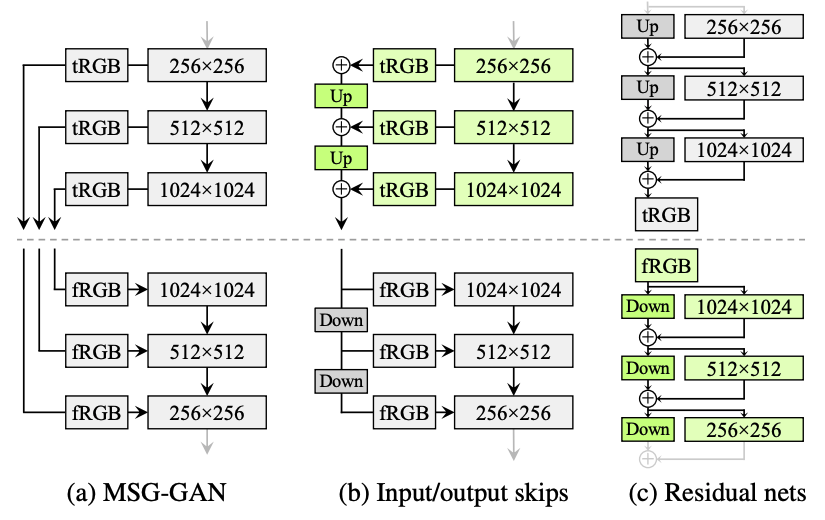
\includegraphics[width=0.7\columnwidth]{XCsD745.png}

\end{column}
\end{columns}


\end{frame}

\begin{frame}{Training GANs with limited data (Karras et al, 2020)}

\begin{columns}
\begin{column}{0.5\textwidth}

\begin{itemize}
 \item Previous StyleGAN2 model needed large number of images for training ($\approx$70,000)
 
 \vspace{2em} 
 
 \item Aim: Enable training on limited datasets (1000 images) through data-augmentation

 \vspace{2em} 
 
 \item Problem: augmentations leak into the generated images 

 \vspace{2em} 
 
 \item This is mitigated by ensuring augmentation probability $p$ is lower than a threshold ($\approx$ 0.9). 
 
\begin{center} 
 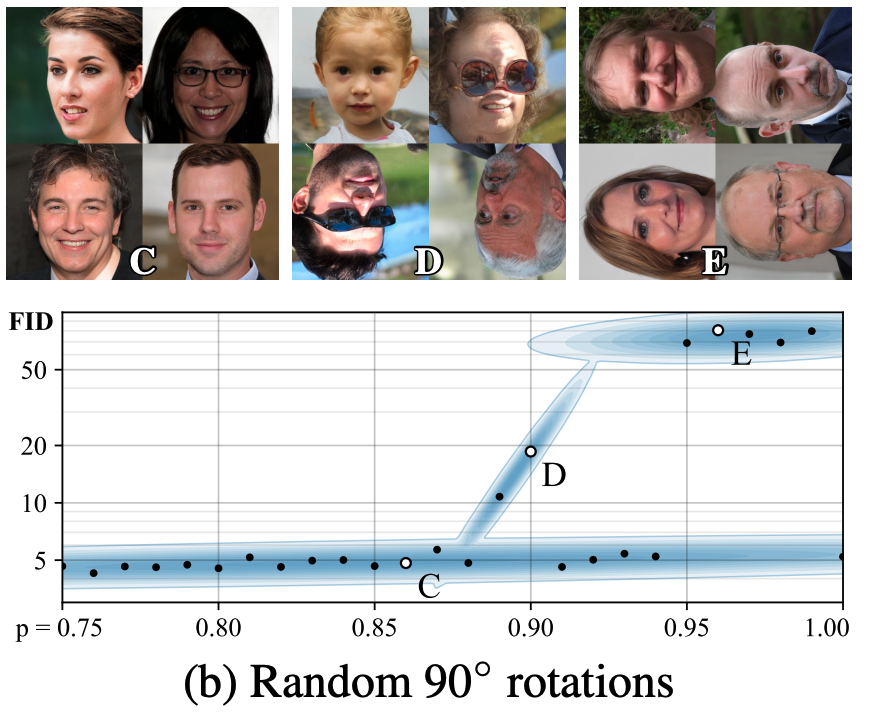
\includegraphics[width=0.5\textwidth]{6H58wvx.png}
\end{center}

\end{itemize}
\end{column}
\begin{column}{0.5\textwidth}
\centering

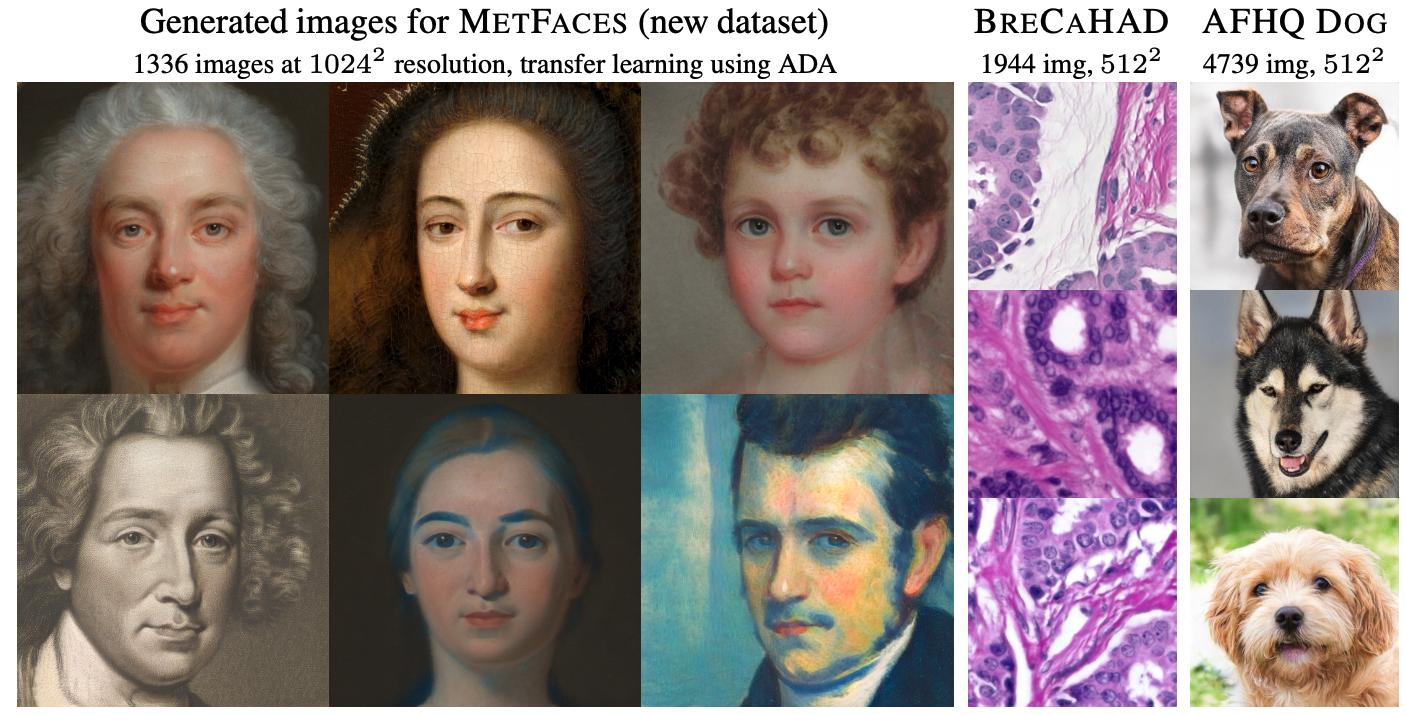
\includegraphics[width=\textwidth]{s4QcxZ4.jpg}

\vspace{2em}

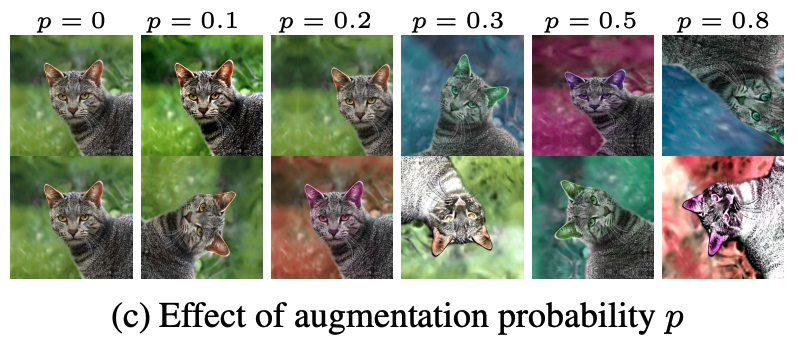
\includegraphics[width=0.8\textwidth]{KBfO0EF.png}
\end{column}
\end{columns}



\end{frame}

\begin{frame}[plain, c]

\begin{center}
\Huge Applications of GANs and other generative models
\end{center}

\end{frame}

\begin{frame}{Application 1: Image super-resolution}

\begin{figure}
\centering
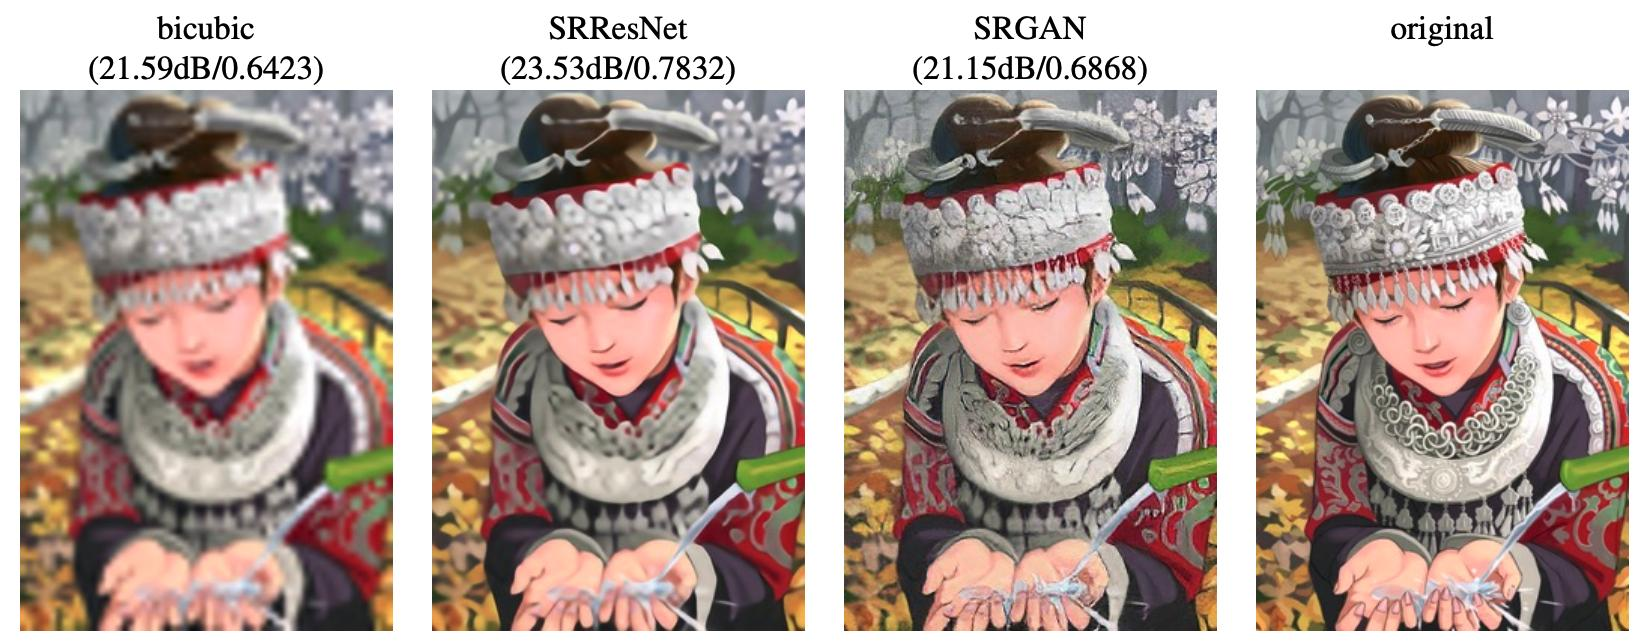
\includegraphics[width=0.9\textwidth]{mVwQduX.jpg}

(Ledig et. al., 2017)
\end{figure}

\begin{itemize}
\item $G$ generates high-res image from low-res input 
\item $D$ discriminates whether high-res image is fake or real. 
\end{itemize}

\end{frame}

\begin{frame}{Application 2: In-painting}

\begin{figure}
\centering
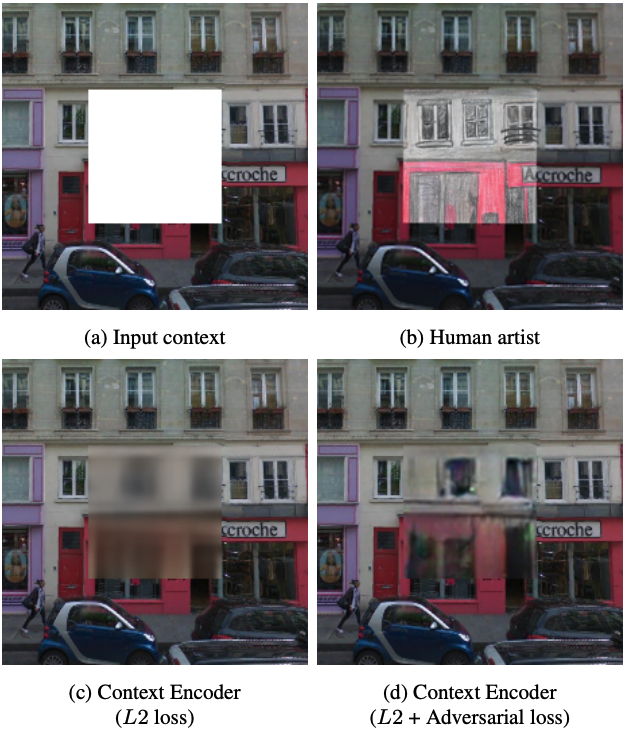
\includegraphics[width=0.4\textwidth]{jVHlxgt.png}

(Pathak et al, 2016)
\end{figure}

\end{frame}

\begin{frame}{Application 3: Image-to-image translation}

\begin{figure}
\centering
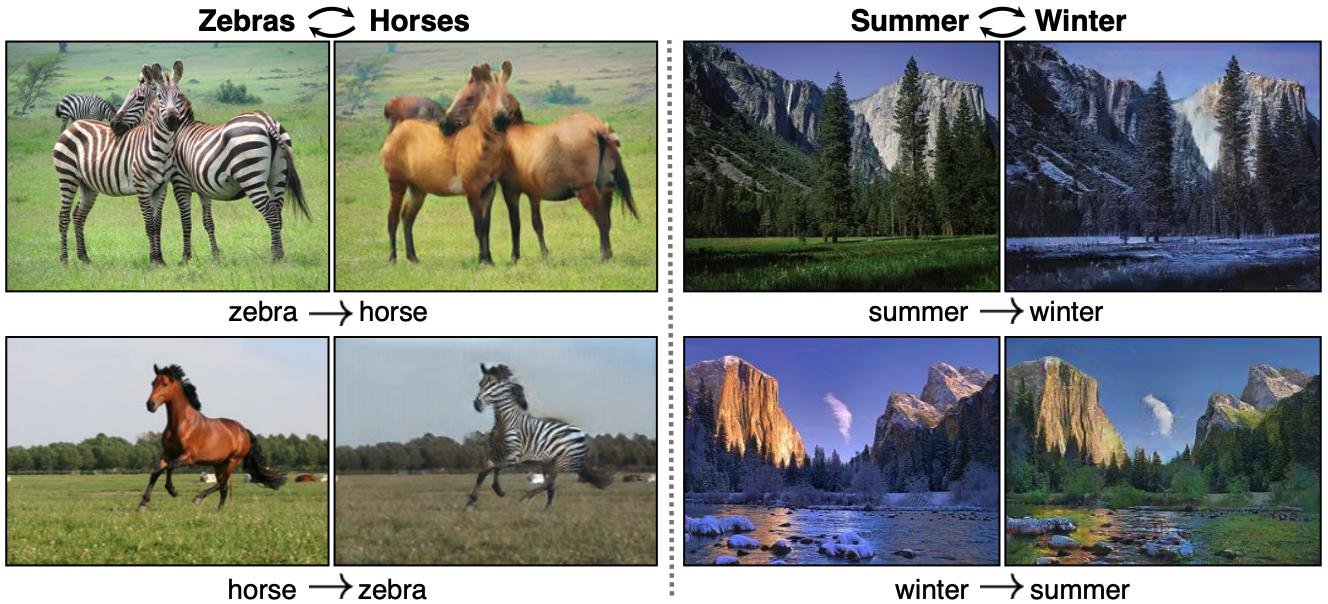
\includegraphics[width=0.8\textwidth]{nxAE9YJ.jpg}

CycleGAN (Jun-Yan Zhu, CVPR, 2016)
\end{figure}

\end{frame}

\begin{frame}{Applications in medical imaging}

\begin{columns}
\begin{column}{0.5\textwidth}
\centering
MRI super-resolution (Sanchez et al., 2018)
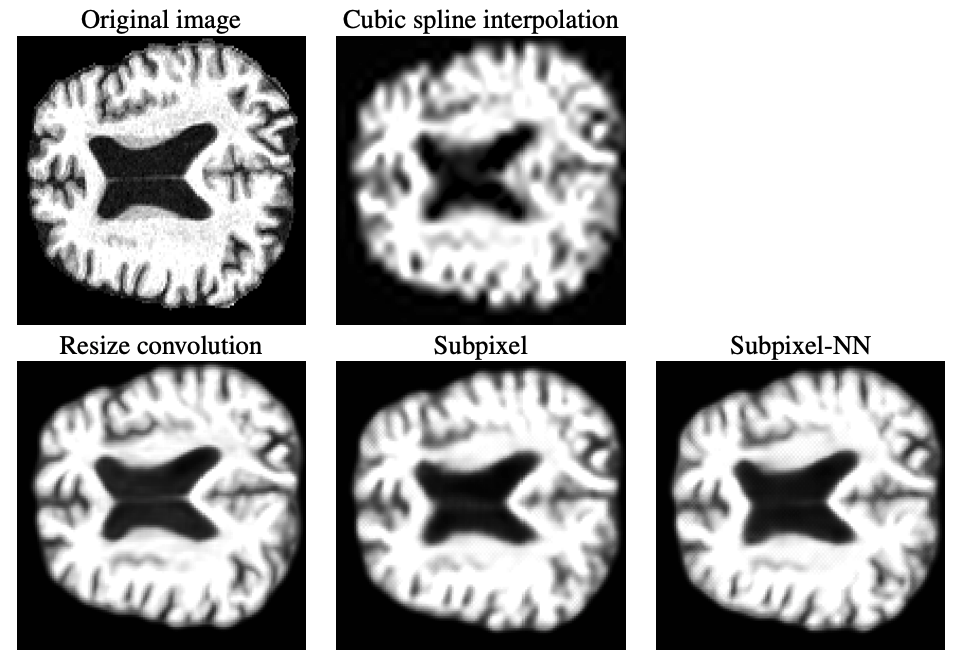
\includegraphics[width=0.5\textwidth]{X6IAL27.png}

\vspace{2em}

Modality translation (Zhang et al, 2019)
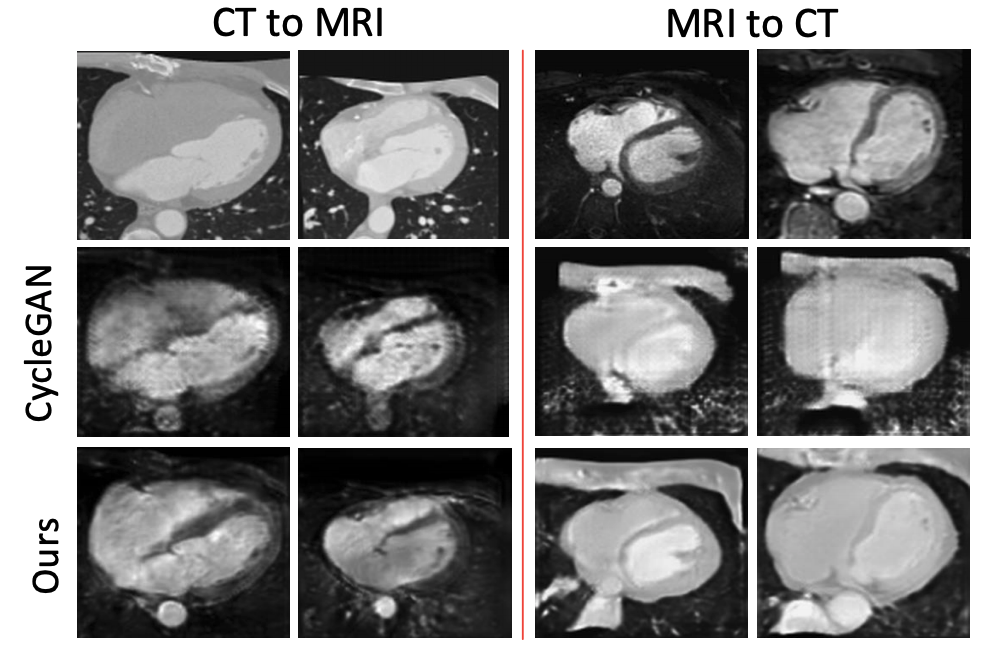
\includegraphics[width=0.5\textwidth]{bJiu3sB.png}


\end{column}
\begin{column}{0.5\textwidth}
\centering
MR Reconstruction from undersampled K-space\\
(Quan et al, 2017, Yang et al, 2017)
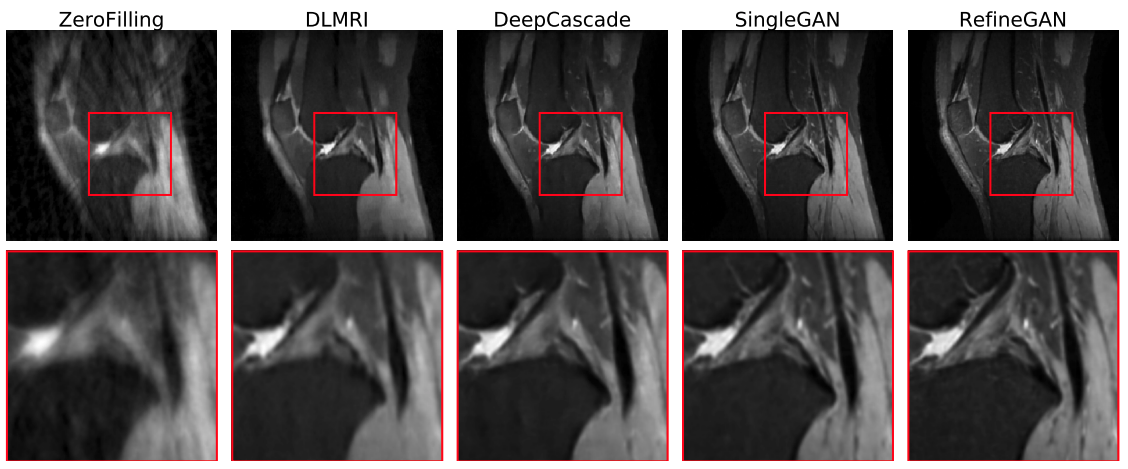
\includegraphics[width=0.6\textwidth]{FGjJDse.png}

\vspace{2em}

MRI motion correction (Usman et al, 2020)
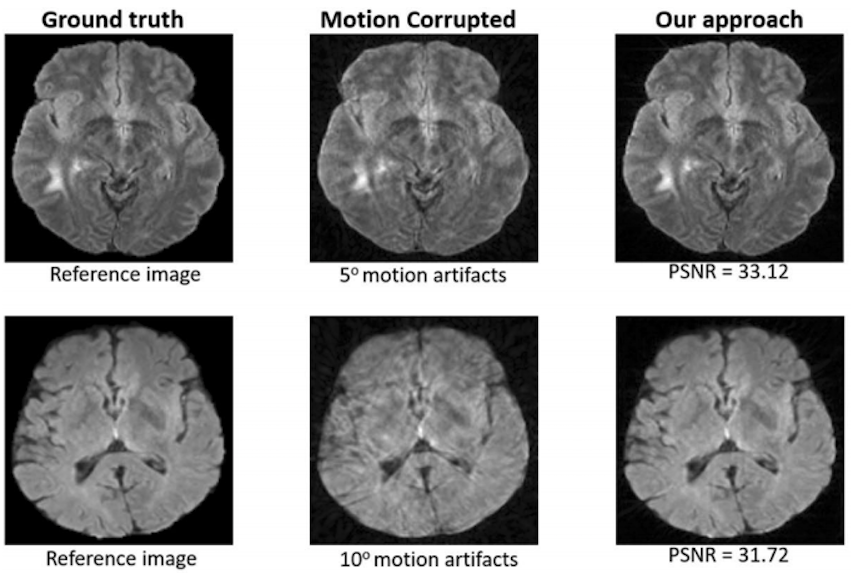
\includegraphics[width=0.6\textwidth]{enijS65.png}


\end{column}
\end{columns}

\begin{center}
Any image reconstruction task!
\end{center}


\end{frame}

\begin{frame}{Applications of generative models to medicine: prediction of disease progression}

\begin{itemize}
\item Prediction and visualisation of future of disease progression
\item Can assist doctors in assigning treatments
\end{itemize}
\vspace{2em}

\begin{columns}
\begin{column}{0.5\textwidth}
\centering
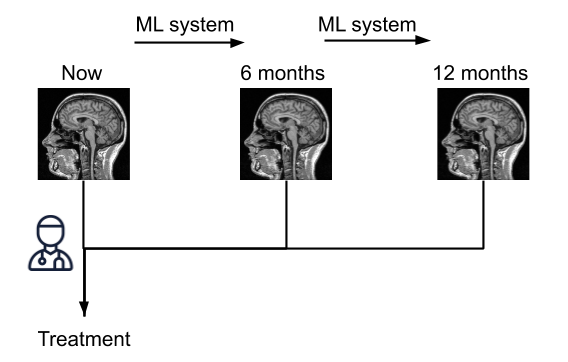
\includegraphics[width=0.8\textwidth]{disprog}
\end{column}
\begin{column}{0.5\textwidth}
\centering
Alzheimer's disease prediction (Ravi et. al., 2019)
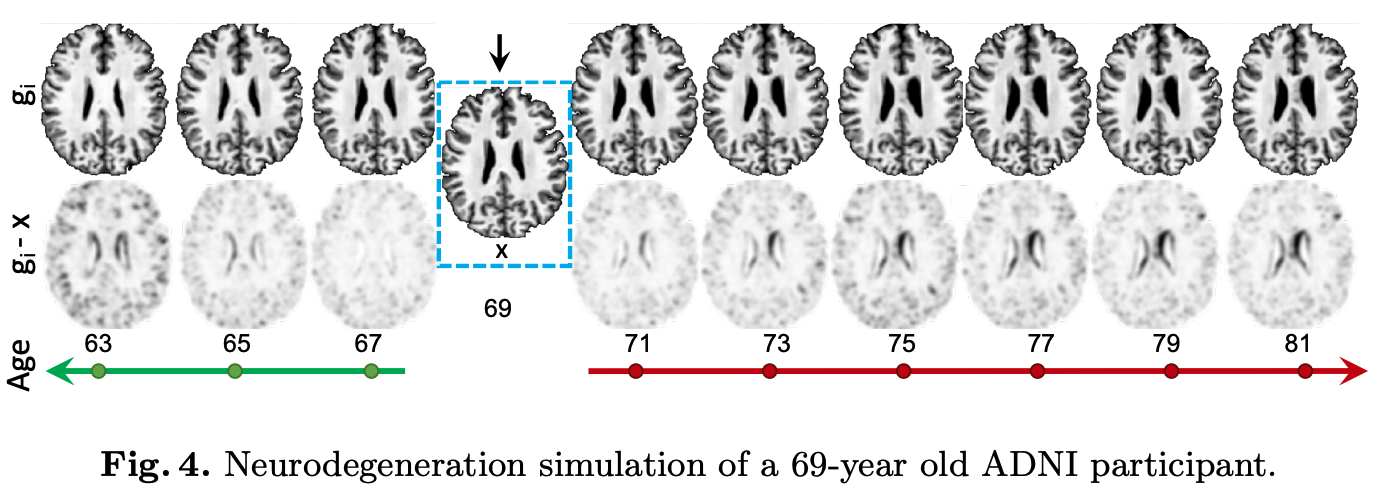
\includegraphics[width=\textwidth]{JFP3eyw.png}
\end{column}
\end{columns}

\end{frame}

\begin{frame}[plain, c]

\begin{center}
\Huge Preliminary results of StyleGAN2 on three medical datasets
\end{center}

\end{frame}


\begin{frame}{Preliminary results of StyleGAN2 on Chest X-rays}
\begin{columns}
\begin{column}{0.5\textwidth}
\centering
Real data
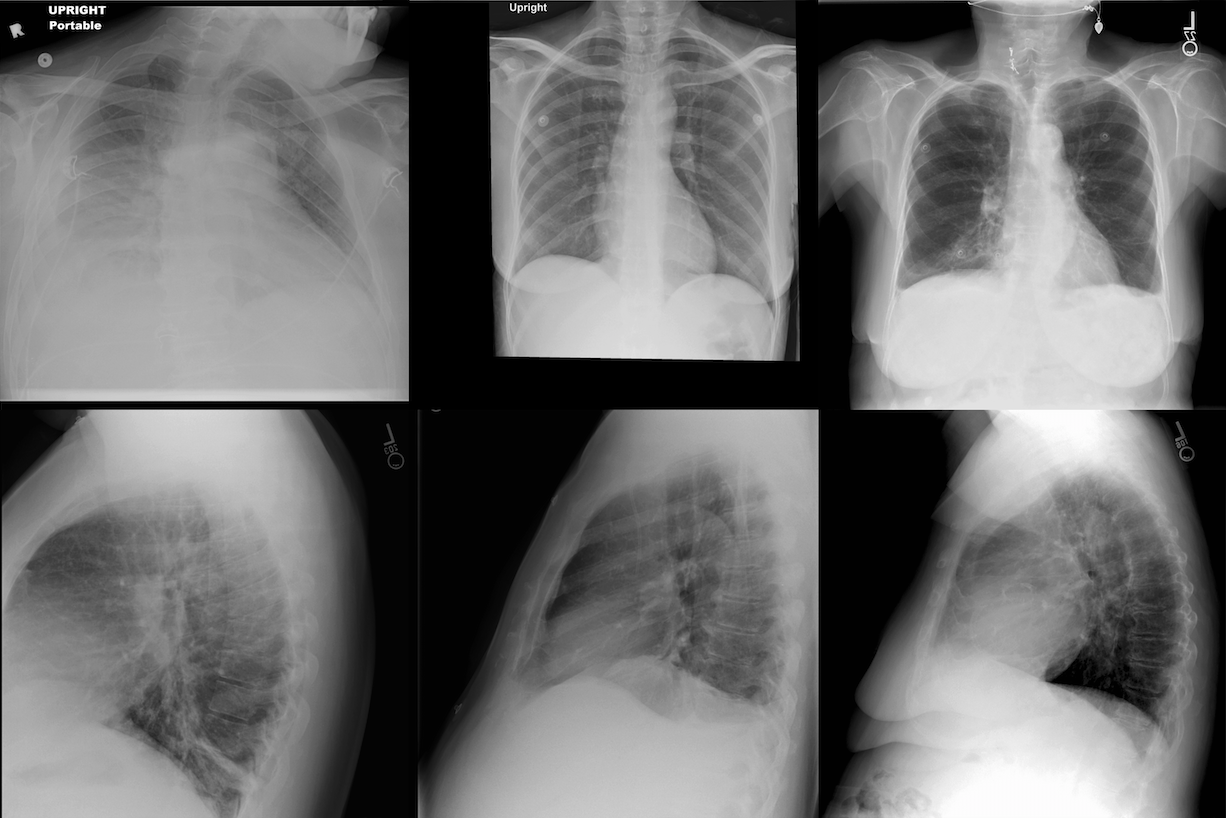
\includegraphics[width=\textwidth]{hhpMkd8.png}
\end{column}
\begin{column}{0.5\textwidth}
\centering
Synthetic data (FID = 23.43, IS=2.4176) % 00037/fakes005038
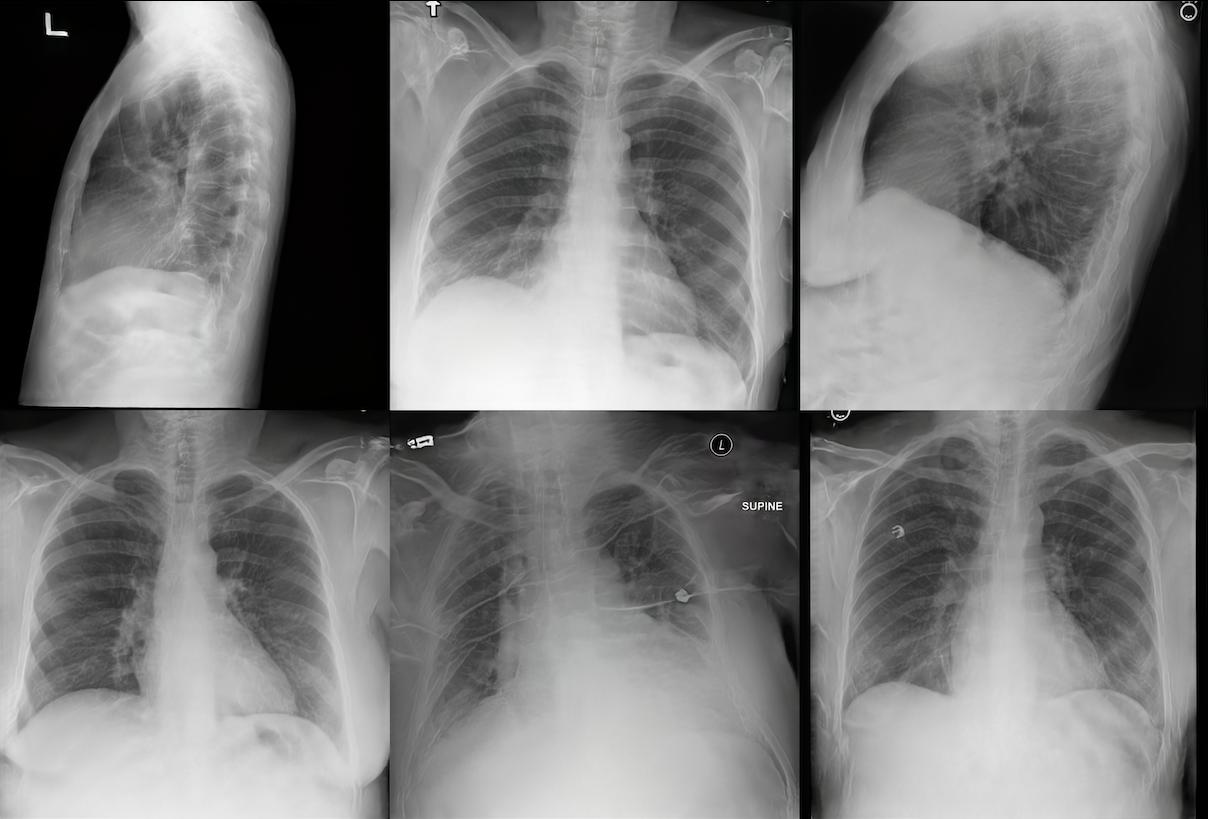
\includegraphics[width=\textwidth]{Z0XeRg3.jpg} % 00037/fakes005038
\end{column}
\end{columns}

\begin{itemize}
\item StyleGAN2 out-of-the box
\item Trained on MIMIC III, 360k images of 1024x1024 resolution
\item Still some problems to fix:
  \begin{itemize}
  \item some ribs look "broken"
  \item bone contours are not always smooth/straight
  \end{itemize}
\end{itemize}
\vspace{1em}

\end{frame}

\begin{frame}{Preliminary results of StyleGAN2 on brain MRI}
\begin{columns}
\begin{column}{0.45\textwidth}
\centering
Real data
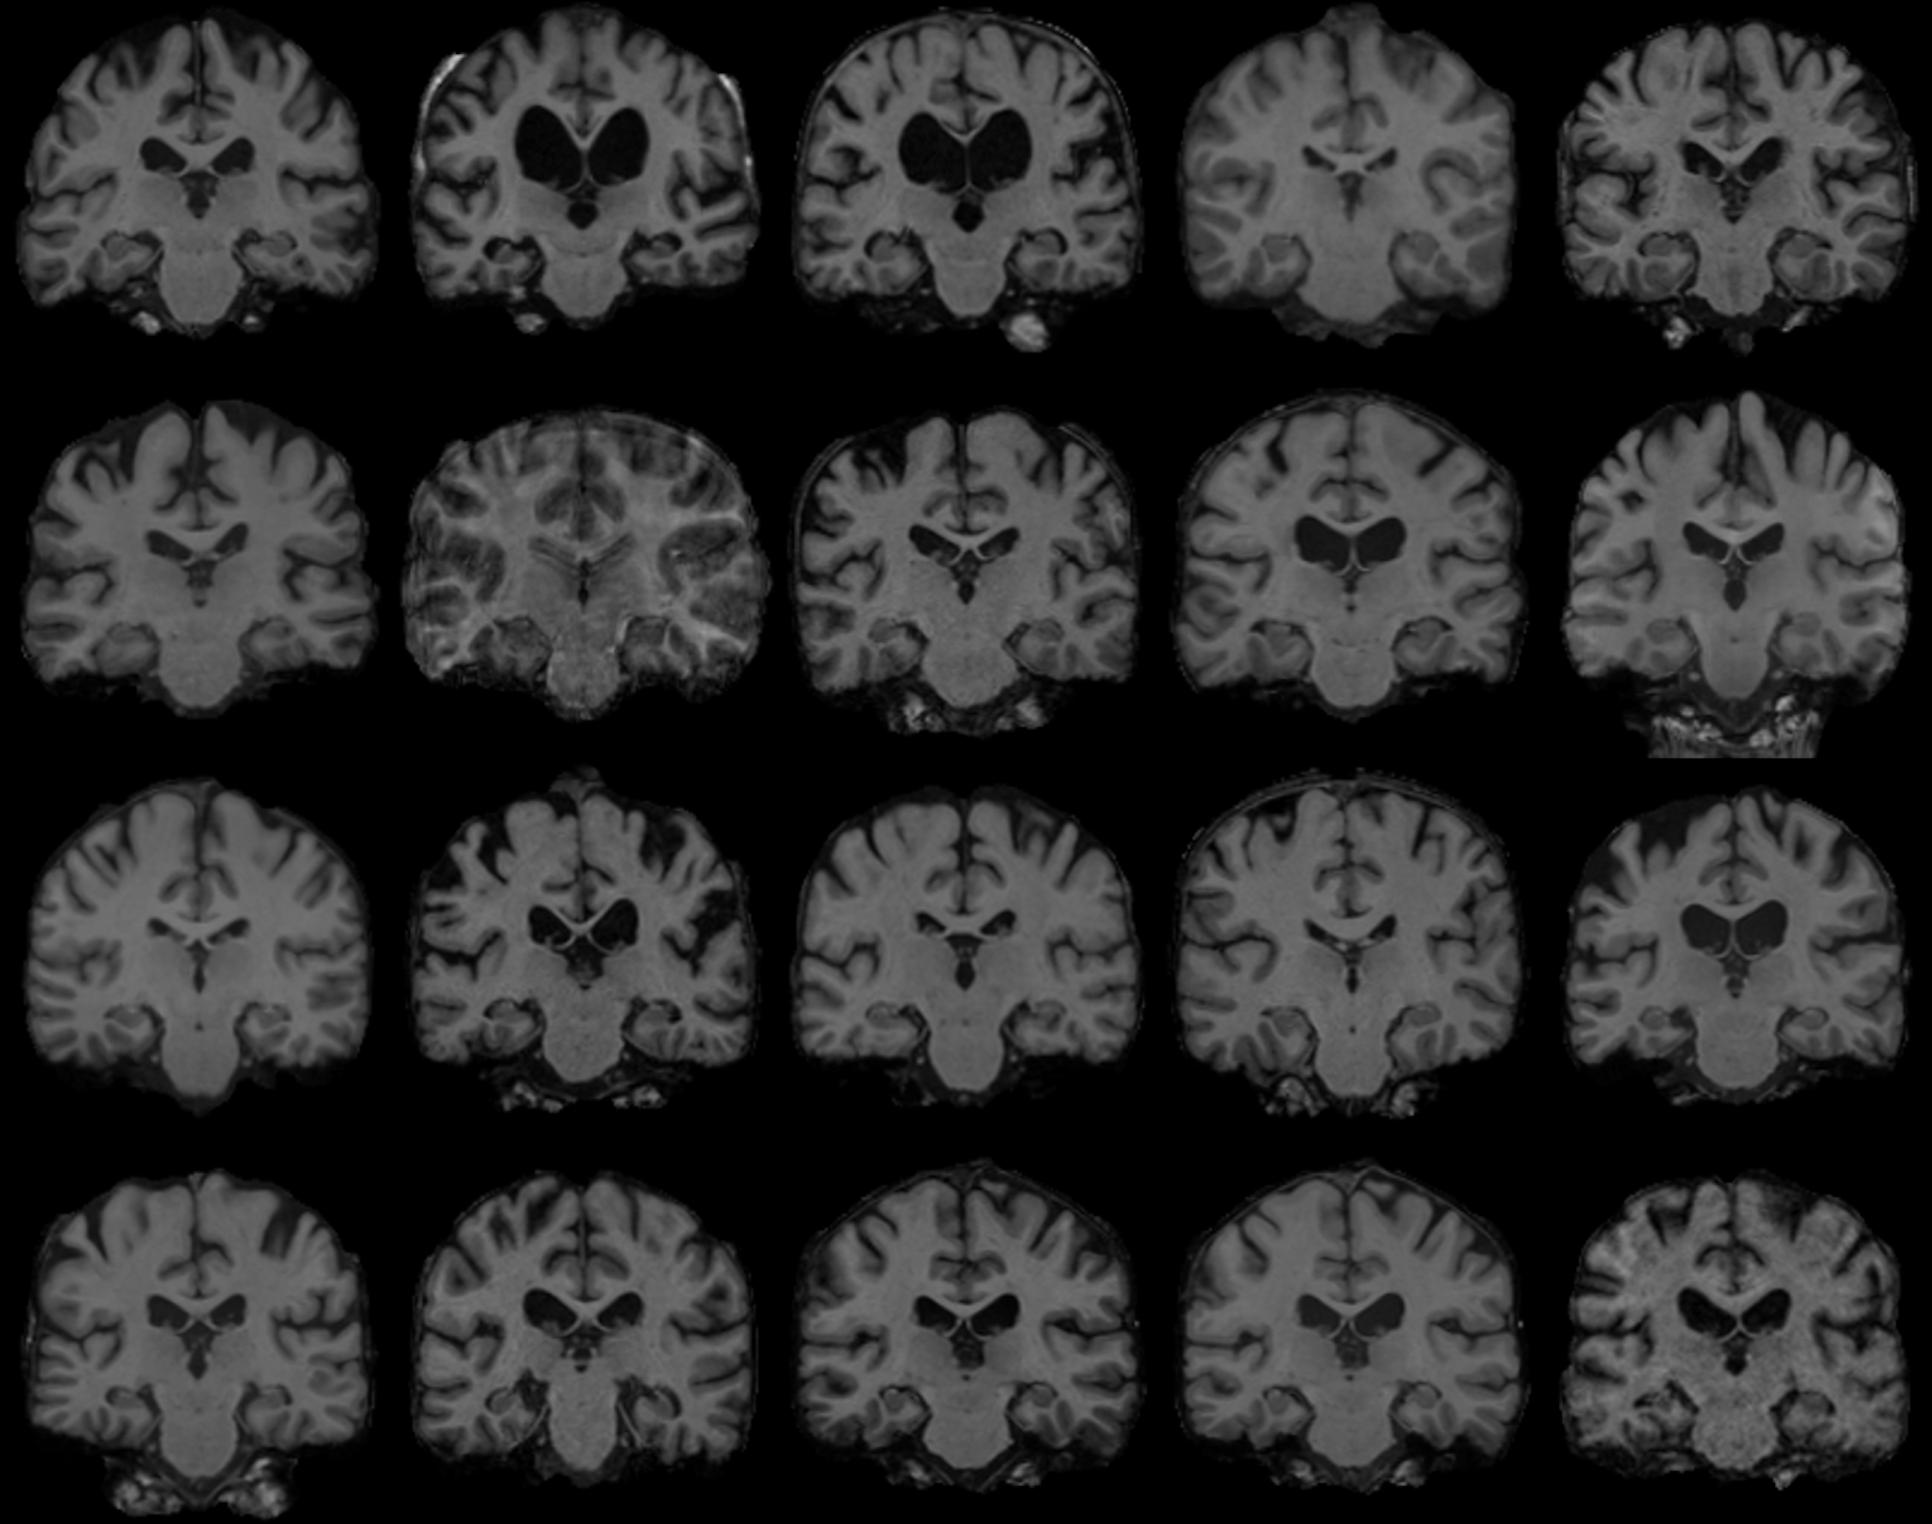
\includegraphics[width=\textwidth]{samY1tk.jpg}
\end{column}
\begin{column}{0.45\textwidth}
\centering
Synthetic data
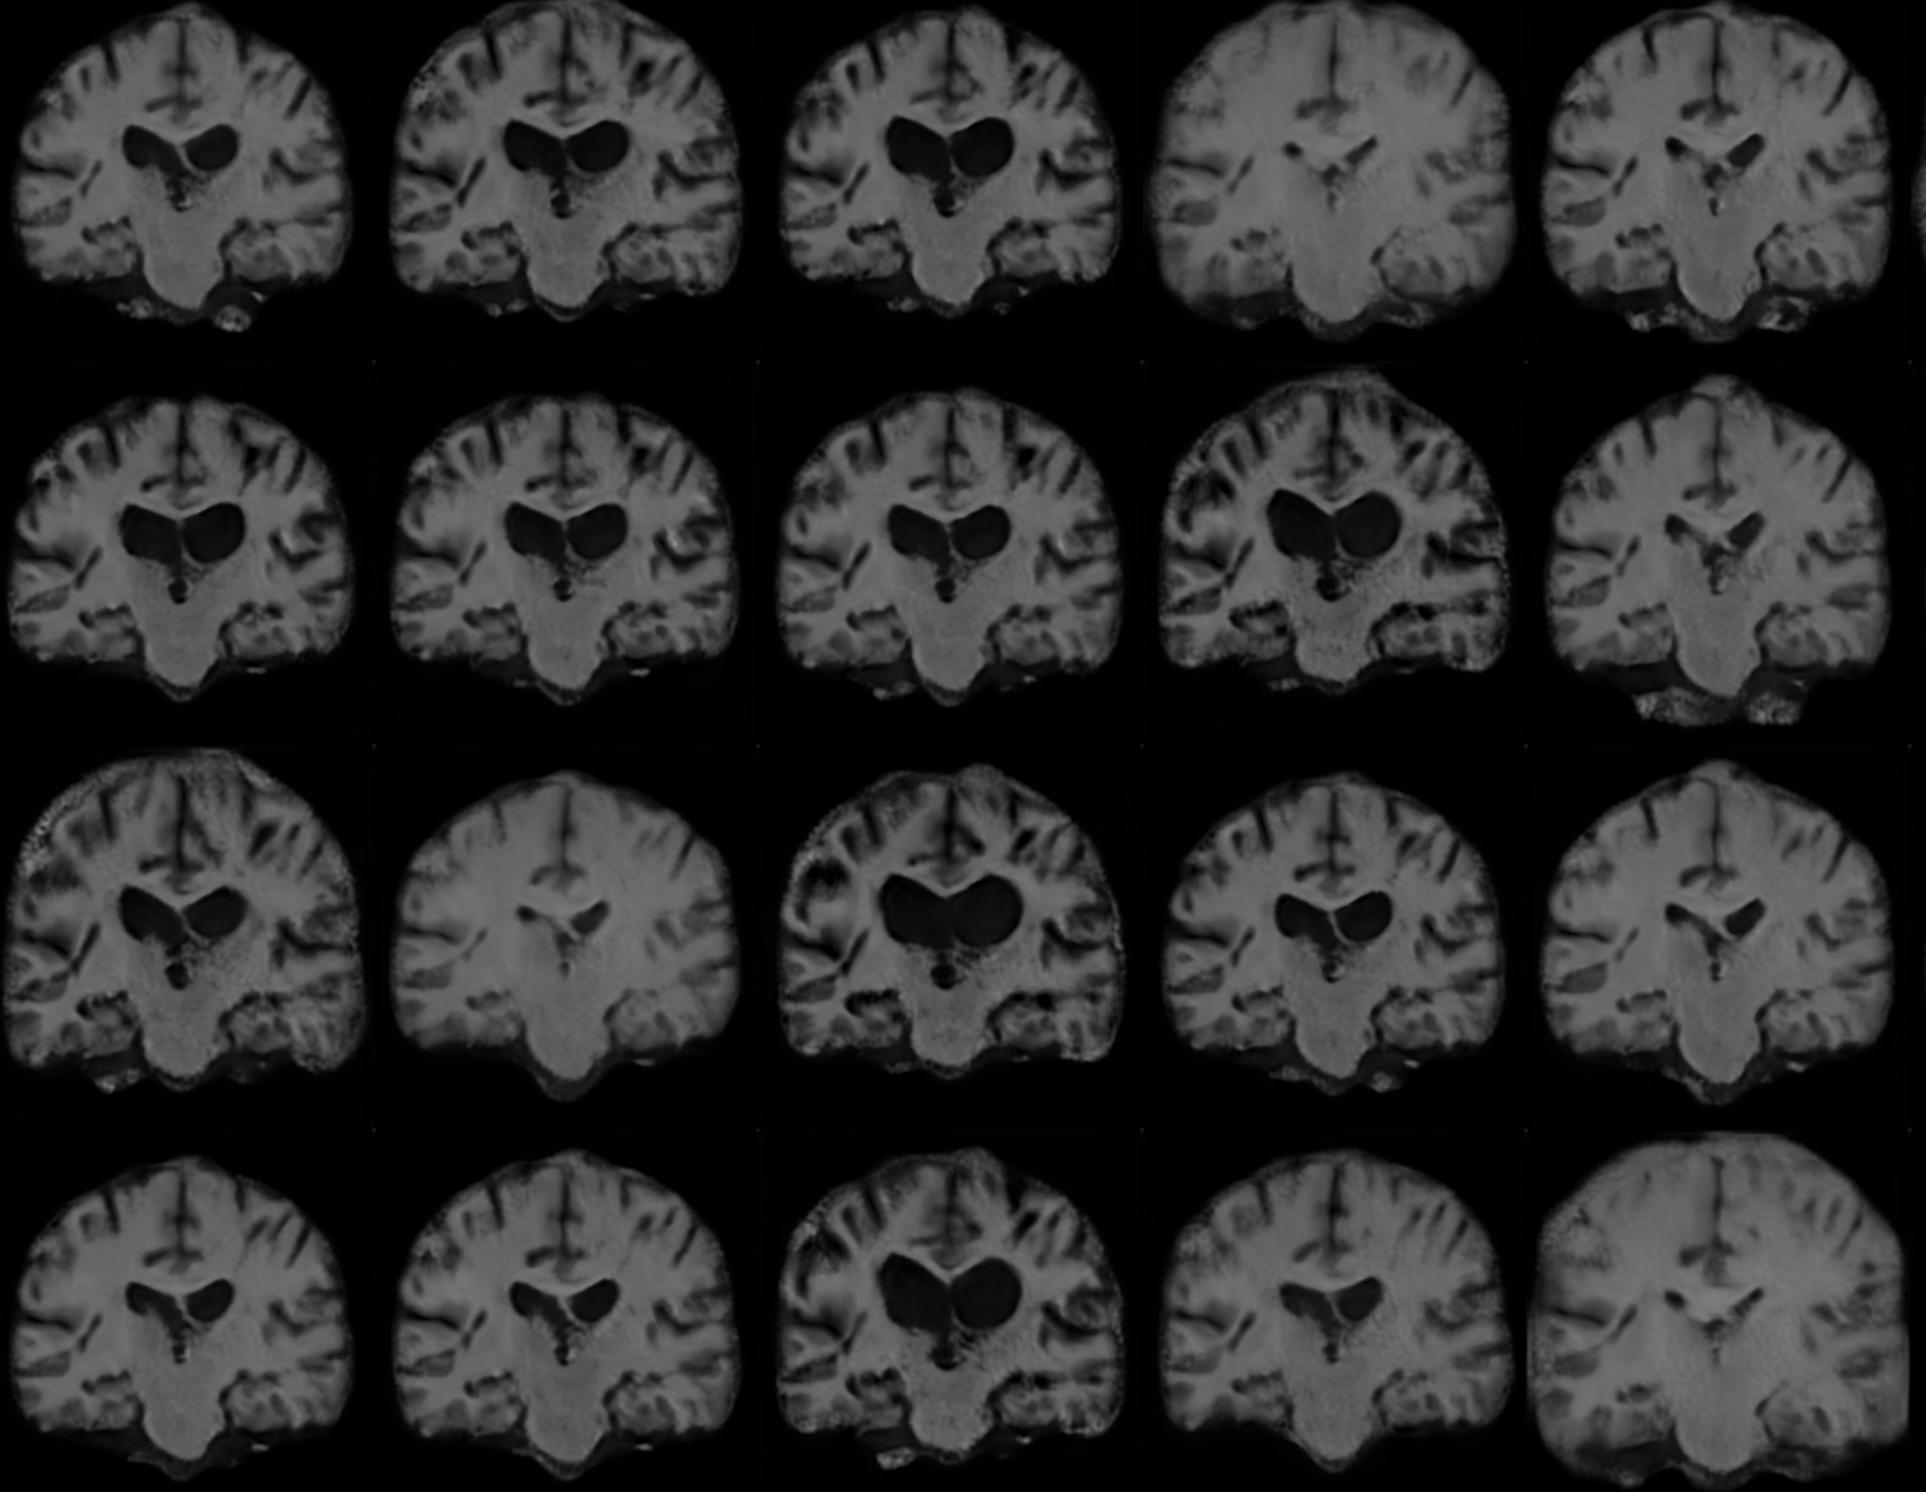
\includegraphics[width=\textwidth]{JvsDI4X.jpg} 
\end{column}
\end{columns}

\begin{itemize}
\item Still out-of-the-box model (StyleGAN2)
\item Trained on 8,000 brain scans (ADNI/OASIS/AIBL/PPMI)
\item Next:
  \begin{itemize}
  \item check if neuroanatomical properties are preserved (e.g. brain/ventricle vols are same)
  \item extend StyleGAN2 to 3D
  \end{itemize}
\end{itemize}
\vspace{1em}

\end{frame}

\begin{frame}{Preliminary results of StyleGAN2 on microscopy images}
\begin{columns}
\begin{column}{0.5\textwidth}
\centering
Real data\\
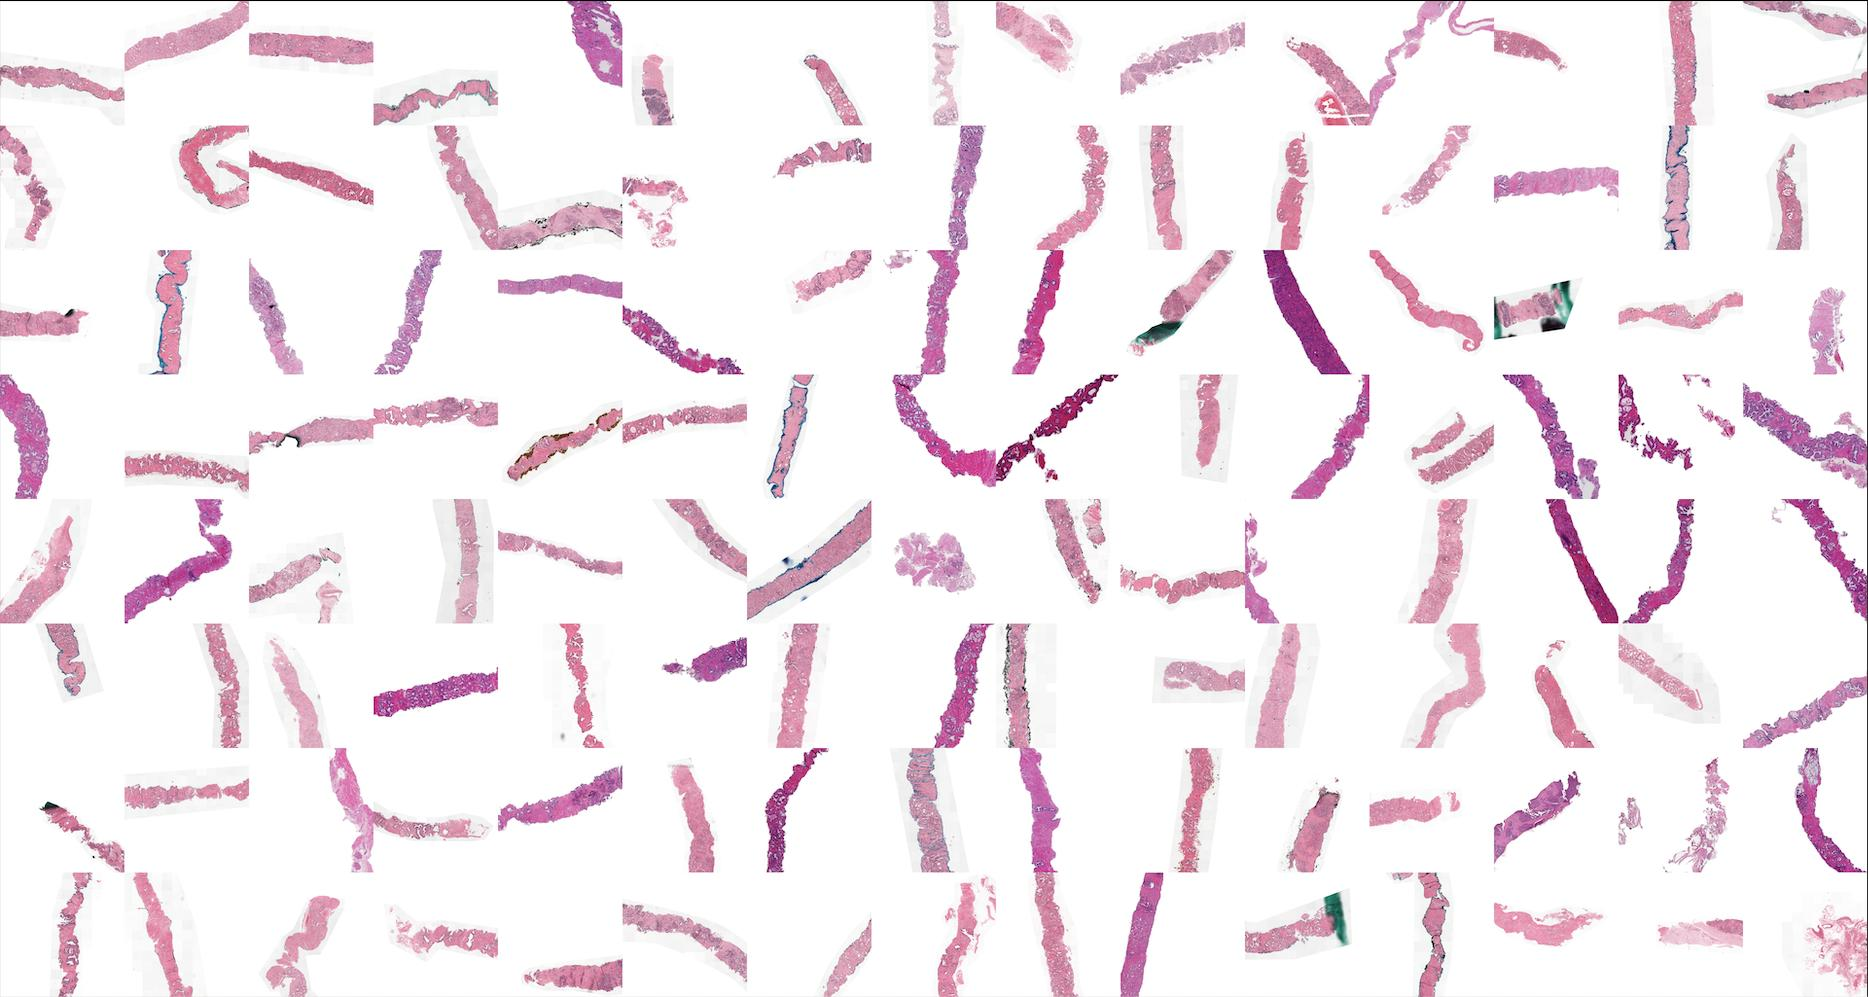
\includegraphics[width=0.7\textwidth]{OlyuTVC.jpg}
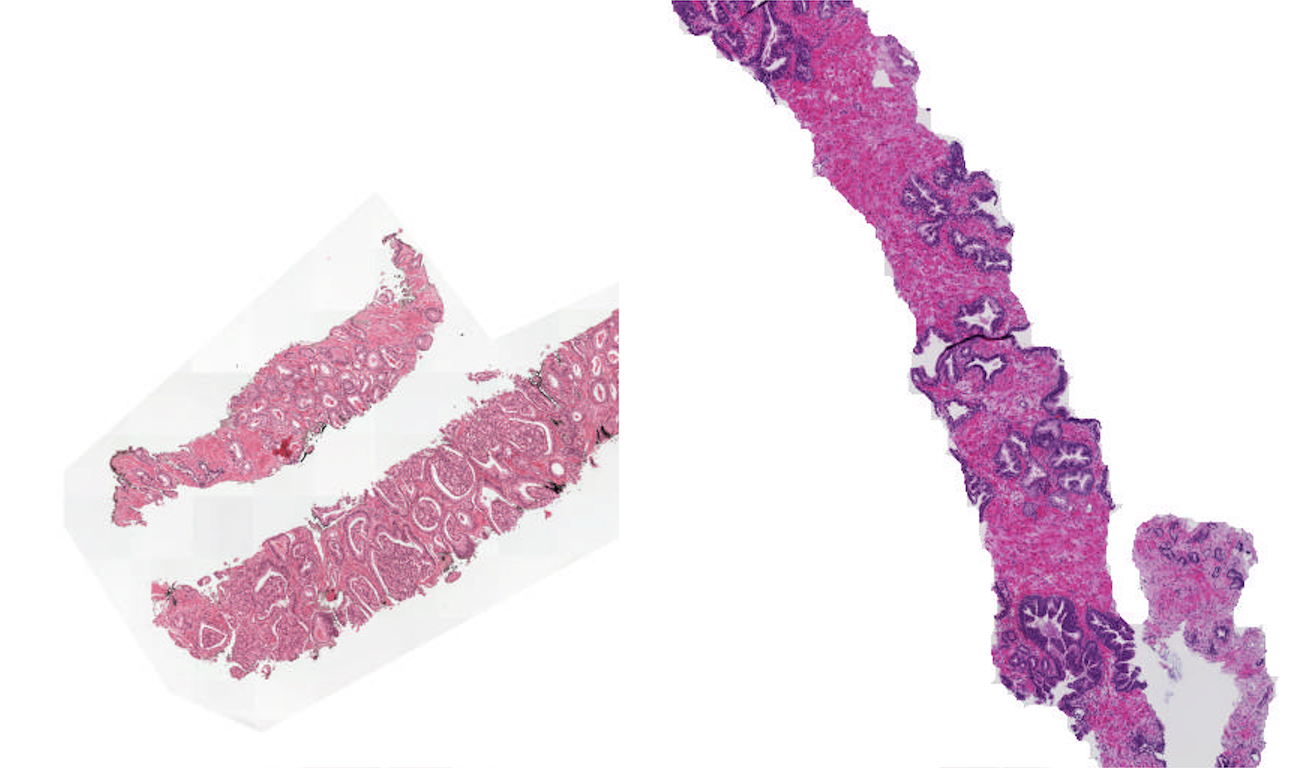
\includegraphics[width=0.7\textwidth]{tzfv0KE.png}
\end{column}
\begin{column}{0.5\textwidth}
\centering
Synthetic data\\

\includegraphics[width=0.7\textwidth]{4GxUSWE.jpg}
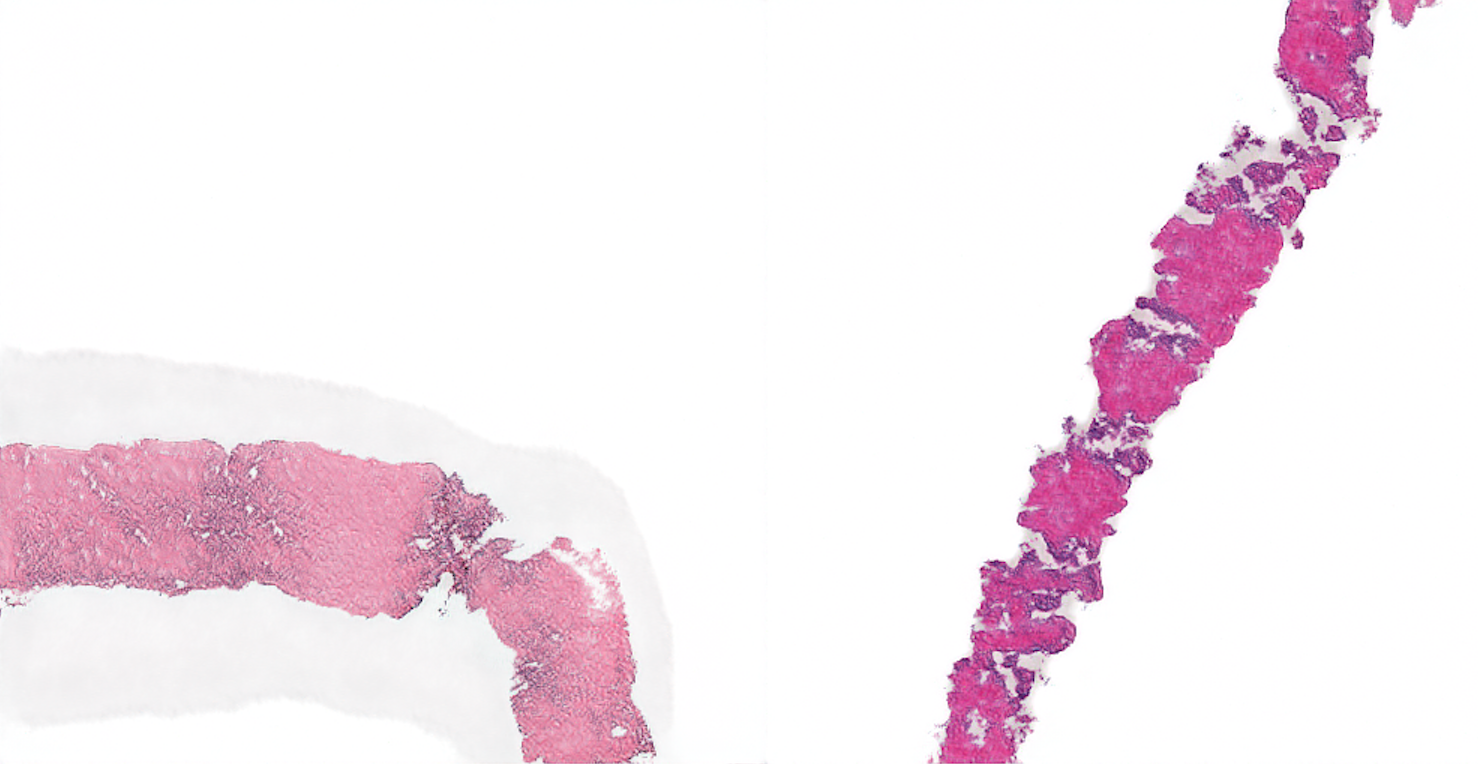
\includegraphics[width=0.7\textwidth]{DDQ740K.png}

\end{column}
\end{columns}

\begin{itemize}
\item Out-of-the-box
\item Trained on 11,000 microscopy slices with pancreatic cancer (MICCAI PANDAS 2020 challenge dataset)
\item 512x512 image crops
\end{itemize}
\vspace{1em}

\end{frame}

\begin{frame}{Conclusion}
\begin{columns}
\begin{column}{0.5\textwidth}
\begin{itemize}
\item GANs have obtained state-of-the-art results on image generation

\vspace{2em}

\item Can generate sharp, realistic images

\vspace{2em}

\item Training now stable compared to 2-3 years ago, but can take up to 6-7 days (StyleGAN2) on 8 GPUs. 

\vspace{2em}

\item Can help solve image reconstruction tasks 

\vspace{2em}

\end{itemize}
\end{column}
\begin{column}{0.5\textwidth}

\begin{itemize}
\item Many potential applications in medical imaging

\vspace{2em}

\item Recommendations:
\begin{itemize}
  \item Don't build your own, start with a state-of-the-art model (StyleGAN2, BigGAN or Karras, 2020)
  \item Download models already pre-trained to explore their capabilities
  \item When training, initialise weights from another pre-trained model instead of random
  \item PIs: Include costs for buying GPUs/AWS-credits in your grant applications 
\end{itemize}

\vspace{2em}

\item Keep an eye on other types of generative models (VAEs, auto-regressive, flow) that have other interesting properties (e.g. density estimation), which enable other tasks e.g. anomaly detection

\end{itemize}

\end{column}
\end{columns}

\end{frame}



\end{document}



